% =============================================================================
% Informe técnico – INFB8091 Desempeño de Sistemas (UTEM, 2026-2)
% Proyecto: Subligol (comercio electrónico de insumos de sublimación)
%
% Compilar desde esta carpeta:  latexmk -pdf informe.tex
% Gráficos:   ../carga/graficos/        (python3 carga/graficos.py)
% Capturas:   ../Capturas configuracion/ (GA4 y Tag Manager)
% Los textos marcados con \pendiente{...} (en rojo) faltan por completar.
% =============================================================================
\documentclass[11pt,a4paper]{article}

\usepackage[utf8]{inputenc}
\usepackage[T1]{fontenc}
\usepackage[spanish,es-tabla,es-nodecimaldot]{babel}
\usepackage{newpxtext}               % texto: Palatino
\usepackage{newpxmath}               % matemáticas a juego
\usepackage{lastpage}
\usepackage[margin=2.3cm,top=2.8cm]{geometry}
\usepackage{graphicx}
\usepackage{booktabs}
\usepackage{tabularx}
\usepackage{array}
\usepackage{float}
\usepackage{caption}
\usepackage{subcaption}
\usepackage[table]{xcolor}
\usepackage{enumitem}
\usepackage{etoolbox}
\usepackage{needspace}
\usepackage{tikz}
\usetikzlibrary{positioning,fit,arrows.meta}
\usepackage[most]{tcolorbox}
\usepackage{titlesec}
\usepackage{titletoc}
\usepackage{fancyhdr}
\usepackage[hidelinks]{hyperref}
\usepackage{xurl}

% --- Colores (Manual de Identidad Visual UTEM) --------------------------------
\definecolor{azulutem}{RGB}{0,78,170}
\definecolor{verdeutem}{RGB}{120,191,38}
\definecolor{azulclaro}{RGB}{232,240,250}
\definecolor{verdeclaro}{RGB}{241,248,232}
\definecolor{grisfila}{RGB}{244,246,249}
\definecolor{gristexto}{RGB}{90,98,110}

% --- Títulos: versalitas con número separado por una barra -------------------
\titleformat{\section}{\Large\scshape\color{azulutem}}
  {\thesection\enspace{\color{gristexto}\textbar}}{0.6em}{}
  [\vspace{0.15em}{\color{gristexto}\titlerule[0.4pt]}]
\titleformat{name=\section,numberless}{\Large\scshape\color{azulutem}}{}{0pt}{}
  [\vspace{0.15em}{\color{gristexto}\titlerule[0.4pt]}]
\titleformat{\subsection}{\large\bfseries\color{azulutem!80!black}}
  {\thesubsection}{0.8em}{}
\titlespacing*{\section}{0pt}{1.6em}{0.9em}
% Un título nunca queda solo al pie de la página
\pretocmd{\section}{\Needspace{0.28\textheight}}{}{}
\pretocmd{\subsection}{\Needspace{0.18\textheight}}{}{}

% --- Índice -------------------------------------------------------------------
\titlecontents{section}[2.2em]{\addvspace{0.5em}\scshape\color{azulutem}}
  {\contentslabel{2.2em}}{}{\hfill\contentspage}
\titlecontents{subsection}[4.6em]{\color{gristexto}}
  {\contentslabel{2.4em}}{}{\titlerule*[0.6pc]{.}\contentspage}

% --- Encabezado y pie ---------------------------------------------------------
\pagestyle{fancy}
\fancyhf{}
\fancyhead[L]{\small\scshape\color{gristexto}Informe técnico · Desempeño de Subligol}
\fancyhead[R]{
\includegraphics[height=0.6cm]{logo-utem.png}}
\fancyfoot[L]{\small\color{gristexto}INFB8091 Desempeño de Sistemas · UTEM 2026-2}
\fancyfoot[R]{\small\color{gristexto}Página \thepage\ de \pageref*{LastPage}}
\renewcommand{\headrulewidth}{0.4pt}
\renewcommand{\headrule}{\hbox to\headwidth{\color{gristexto}\leaders\hrule height \headrulewidth\hfill}}
\setlength{\headheight}{24pt}
\fancypagestyle{plain}{\fancyhf{}\fancyfoot[R]{\small\color{gristexto}Página \thepage\ de \pageref*{LastPage}}\renewcommand{\headrulewidth}{0pt}}

% --- Tablas: estilo clásico (booktabs) ----------------------------------------
\renewcommand{\arraystretch}{1.15}

% --- Recuadros de resultados clave --------------------------------------------
\newtcolorbox{clave}[1][Resultados clave]{enhanced, breakable, sharp corners,
  colback=white, colframe=gristexto, boxrule=0.4pt, leftrule=0.4pt,
  left=10pt, right=10pt, top=6pt, bottom=6pt,
  fonttitle=\scshape, coltitle=azulutem, colbacktitle=white,
  attach title to upper={\par\smallskip}, title=#1}

\graphicspath{{./}{../carga/graficos/}{../Capturas configuracion/}}
\captionsetup{font=small,labelfont={bf,sc}}
\setlist{itemsep=2pt,topsep=4pt}
\setlist[itemize,1]{label={\color{azulutem}\textbullet}}
\newcommand{\pendiente}[1]{\textcolor{red}{\textbf{[PENDIENTE: #1]}}}
\newcommand{\codigo}[1]{\texttt{#1}}
\newcolumntype{R}{>{\raggedleft\arraybackslash}X}

% --- RUT de los integrantes ----------------------------------------------------
% Los RUT no se publican en el repositorio. Están en ruts.tex (excluido por
% .gitignore) y solo se incluyen en la versión de entrega:
%   latexmk -pdf informe.tex                          -> informe.pdf (sin RUT, público)
%   latexmk -pdf -jobname=informe-entrega informe.tex -> informe-entrega.pdf (con RUT)
\newcommand{\rutWladimir}{}\newcommand{\rutRodrigo}{}\newcommand{\rutLeonardo}{}
\ifnum\pdfstrcmp{\jobname}{informe-entrega}=0
  \IfFileExists{ruts.tex}{\input{ruts.tex}}{\PackageWarning{informe}{Falta ruts.tex}}
\fi

\begin{document}

% -----------------------------------------------------------------------------
% Portada: franja lateral azul (Manual de Identidad Visual UTEM)
% -----------------------------------------------------------------------------
\newgeometry{left=3.4cm,right=2.5cm,top=2.5cm,bottom=2.5cm}
\begin{titlepage}
  \thispagestyle{empty}
  \noindent\begin{tikzpicture}[remember picture, overlay]
    \fill[azulutem] (current page.north west) rectangle ([xshift=1.1cm]current page.south west);
    \fill[verdeutem] ([xshift=1.1cm]current page.north west) rectangle ([xshift=1.2cm]current page.south west);
  \end{tikzpicture}%
  \raggedright
  
\includegraphics[width=6.5cm]{logo-utem.png}\par
  \vspace{0.3cm}
  {\color{gristexto}Facultad de Ingeniería\par}
  \vspace{3.2cm}
  {\large\scshape\color{gristexto}Informe técnico · Trabajo Semestre 2, 2026\par}
  \vspace{0.5cm}
  {\color{azulutem}\rule{\linewidth}{0.8pt}\par}
  \vspace{0.5cm}
  {\fontsize{26}{32}\selectfont\color{azulutem} Análisis de desempeño\\de Subligol bajo carga\par}
  \vspace{0.5cm}
  {\Large\itshape\color{gristexto} Un comercio electrónico medido con GA4, k6 y Prometheus\par}
  \vspace{0.5cm}
  {\color{azulutem}\rule{\linewidth}{0.8pt}\par}
  \vspace{0.4cm}
  {\large INFB8091 -- Desempeño de Sistemas\par}
  \vfill
  \renewcommand{\arraystretch}{1.25}
  \begin{tabular}{@{}l l l@{}}
    \textsc{Integrantes} & Wladimir Gallardo & \rutWladimir \\
                 & Rodrigo Donoso    & \rutRodrigo \\
                 & Leonardo Solís    & \rutLeonardo \\[6pt]
    \textsc{Profesor}    & Javier Aranda & \\[6pt]
    \textsc{Fecha}       & Lunes 16 de noviembre de 2026 &
  \end{tabular}\par
  \vspace{0.8cm}
  {\small\color{gristexto}
  Sitio: \url{https://subligol-utem.chilecentral.cloudapp.azure.com}\\
  Repositorio: \url{https://github.com/Wlvdi/trabajo-desempeno}\par}
\end{titlepage}
\restoregeometry

\tableofcontents
\newpage

% -----------------------------------------------------------------------------
\section*{Resumen ejecutivo}
\addcontentsline{toc}{section}{Resumen ejecutivo}

\begin{tcolorbox}[enhanced, sharp corners, colback=white, colframe=gristexto,
  boxrule=0pt, toprule=0.4pt, bottomrule=0.4pt, left=0pt, right=0pt, top=8pt, bottom=8pt,
  before upper={\setlength{\parskip}{0.6em}}]
Se construyó \textbf{Subligol}, una tienda en línea de insumos de sublimación e
impresión (catálogo de 500 productos, búsqueda, carrito, registro, checkout con
pago simulado y con Webpay Plus en ambiente de integración), instrumentada con
Google Analytics 4, Web Vitals y Prometheus/Grafana, y desplegada en una máquina
virtual de Azure (2 vCPU, 7,7~GB). Con k6 se generó tráfico sintético de cuatro
perfiles de usuario (navegación, búsqueda, abandono de carrito y compra) en tres
escenarios (carga baja, normal y estrés), con tres repeticiones cada uno.

Con carga baja y normal el sistema responde holgadamente: p95 de
\textbf{18,5~ms} y \textbf{17,5~ms}, sin errores, con 6 veces más carga en el
escenario normal y sin degradación. En el estrés escalonado la latencia crece de
forma no lineal desde \textbf{$\sim$40~sesiones/s ($\sim$155~req/s)}: la CPU de la
VM llega al 95~\% y el p95 salta de 117~ms a 705~ms. El criterio de saturación
(p95~>~800~ms o logrado~<~90~\%) se cruza en \textbf{50~sesiones/s}, con un
throughput máximo de \textbf{$\sim$172~req/s}. \textbf{El recurso limitante es la
CPU de la VM}, compartida por la API (Node.js) y PostgreSQL; una sola consulta
(productos relacionados del detalle) consume el \textbf{79~\%} del tiempo de la
base de datos y es la principal propuesta de mejora. La ley de utilización
predijo una capacidad de $\sim$41~sesiones/s, coherente con lo medido (40--45).
\end{tcolorbox}

% -----------------------------------------------------------------------------
\section{Introducción y objetivos}

El objetivo del trabajo es diseñar, implementar y evaluar el desempeño de un
sitio de comercio electrónico bajo distintas condiciones de carga, aplicando
medición, generación de tráfico y análisis cuantitativo de indicadores.
Objetivos específicos:
\begin{enumerate}
  \item Instrumentar una aplicación web real con GA4 (eventos de comercio
        electrónico, engagement y embudo de conversión).
  \item Construir generadores de carga que simulen usuarios concurrentes con
        comportamientos distintos y parametrizables.
  \item Medir latencia (promedio, mediana, p90, p95, p99), throughput, tasa de
        error y utilización de recursos, e identificar el punto de saturación.
  \item Comparar la experiencia de usuario (Web Vitals y GA4) sin carga y bajo carga.
  \item Proponer mejoras basadas en la evidencia.
\end{enumerate}

% -----------------------------------------------------------------------------
\Needspace{0.5\textheight}
\section{Arquitectura del sistema}

\begin{figure}[H]
\centering
\begin{tikzpicture}[
  caja/.style={draw, rounded corners=3pt, align=center, minimum width=2.7cm, minimum height=1cm, font=\small},
  zona/.style={draw, dashed, rounded corners=6pt, inner sep=8pt},
  flecha/.style={-{Stealth[length=2.2mm]}, thick}]
  \node[caja] (nav) {Navegador\\(React + Vite)};
  \node[caja, below=0.9cm of nav] (k6) {Generador k6\\(PC del grupo)};
  \node[caja, right=1.6cm of nav] (caddy) {Caddy 2.10\\HTTPS + estáticos};
  \node[caja, right=1.2cm of caddy] (api) {API Node 24\\Express 5};
  \node[caja, right=1.2cm of api] (db) {PostgreSQL 16};
  \node[caja, below=0.9cm of api] (prom) {Prometheus\\+ Grafana};
  \node[caja, below=0.9cm of db, font=\scriptsize] (exp) {node-exporter, cAdvisor,\\postgres-exporter};
  \node[caja, above=0.8cm of nav] (ga) {Google Analytics 4\\(vía Tag Manager)};
  \node[caja, above=0.8cm of db] (tbk) {Webpay Plus\\(integración)};
  \node[zona, fit=(caddy)(api)(db)(prom)(exp), label={[font=\small]below:VM Azure Chile Central · 2 vCPU · 7,7 GB · Docker Compose}] {};
  \draw[flecha] (nav) -- (caddy);
  \draw[flecha] (k6) -| (caddy);
  \draw[flecha] (caddy) -- node[above, font=\scriptsize]{/api} (api);
  \draw[flecha] (api) -- node[above, font=\scriptsize]{pool 10} (db);
  \draw[flecha] (prom) -- (api);
  \draw[flecha] (exp) -- (prom);
  \draw[flecha] (nav) -- (ga);
  \draw[flecha] (api) |- (tbk);
\end{tikzpicture}
\caption{Arquitectura desplegada. El generador de carga corre fuera de la VM.}
\label{fig:arquitectura}
\end{figure}

\begin{table}[H]
\centering\small
\begin{tabularx}{\textwidth}{@{}lX@{}}
\toprule
Componente & Decisión y justificación \\
\midrule
Frontend & React + Vite (JavaScript). SPA servida como archivos estáticos por Caddy. \\
API & Node.js 24 + Express 5. Un solo lenguaje en el sitio y en k6. Contraseñas con argon2id (Biryukov et al., 2016) y sesiones con JWT. \\
Base de datos & PostgreSQL 16 con migraciones propias. Seed de 500 productos, 5 categorías, $\sim$3\,000 ventas históricas y 200 clientes de prueba. La búsqueda queda \emph{sin índices} a propósito, como palanca medible. \\
Pago & Pago simulado (\codigo{mock}, habilitado por variable de entorno) para las pruebas de carga, y Webpay Plus en ambiente de integración de Transbank (Transbank, s.\,f.) para el flujo real con tarjetas de prueba (nunca pasarela real). \\
Observabilidad & prom-client en la API (latencia por ruta, pool, event loop, argon2, compras), node-exporter (VM), cAdvisor (contenedores) y postgres-exporter con \codigo{pg\_stat\_statements} (PostgreSQL Global Development Group, s.\,f.); dashboard de Grafana con 36 paneles (Prometheus Authors, s.\,f.). \\
Infraestructura & VM de Azure (Ubuntu 24.04, 2 vCPU, 7,7~GB) con Docker Compose y Caddy con certificado de Let's Encrypt. Tener la API y la base en una VM propia permite medir CPU, memoria e I/O directamente. \\
\bottomrule
\end{tabularx}
\caption{Componentes y decisiones de diseño.}
\end{table}

\subsection{Proceso de construcción de la tienda}

La tienda se construyó en seis etapas, cada una con su commit, sus tests
automáticos y su \emph{Prompt Card} (sección~\ref{sec:agente}). El criterio que
guió las decisiones fue que todo lo que se quisiera analizar después pudiera
medirse en un servidor propio.

\begin{table}[H]
\centering\small
\begin{tabularx}{\textwidth}{@{}lX@{}}
\toprule
Etapa & Qué se hizo y por qué \\
\midrule
0. Punto de partida &
  Leonardo construyó la tienda en React con catálogo, carrito y panel de
  administración sobre Supabase. Un servicio administrado no deja ver la CPU,
  las consultas ni el pool de conexiones, por lo que se decidió migrar a una API
  propia. \\
1. Configuración (v0.1) &
  \codigo{AGENTS.md}, \codigo{CLAUDE.md}, registro de prompts y archivos base.
  Se fijó la regla de explicar el diseño antes de implementar. \\
2. Backend y datos (v0.2) &
  API en Express 5 y PostgreSQL 16 en Docker, migraciones y datos semilla
  deterministas (500 productos), para que cada prueba parta del mismo estado.
  Las páginas tienen peso distinto a propósito: home liviana, listado media y
  detalle pesada (galería, ventas de 90 días y relacionados). Login con argon2id
  y JWT. \\
3. Compra y métricas (v0.3) &
  Carrito persistente en la base (también anónimo, con fusión al iniciar
  sesión). Checkout en una sola transacción que bloquea los productos en orden
  fijo, para evitar sobreventa y bloqueos mutuos; se probó con 20 compradores
  simultáneos sobre un stock de 5. Pago simulado para las pruebas de carga.
  Métricas de la API con prom-client, Prometheus y Grafana. \\
4. Frontend y GA4 (v0.4) &
  La tienda consume la API propia y se quitó Supabase. GA4 vía Tag Manager con
  los eventos de comercio electrónico, la dimensión \codigo{escenario\_prueba} y
  las Web Vitals, con respaldo en Prometheus. \\
5. Administración (v0.5) &
  Panel protegido por rol (inventario, compras, ventas manuales, dashboard y
  auditoría). Sus rutas no envían eventos a GA4 para no mezclar tráfico interno
  con el de clientes. \\
6. Despliegue y carga (v1.0) &
  VM de Azure con Caddy y HTTPS, generadores k6 y protocolo de ejecución.
  Después se agregó Webpay Plus en ambiente de integración, sin cambiar la
  medición. \\
\bottomrule
\end{tabularx}
\caption{Etapas de construcción del sitio.}
\end{table}

Al terminar la etapa 5 el proyecto tenía 368 tests del backend y 84 del
frontend, incluidos tests de concurrencia del checkout y de las ventas
manuales.

% -----------------------------------------------------------------------------
\section{Uso del agente de codificación}
\label{sec:agente}

Todo el desarrollo se hizo con \textbf{Claude Code} (modelo \textbf{Claude Opus
5.5}) (Anthropic, s.\,f.). Siguiendo el enunciado, el primer prompt configuró \codigo{AGENTS.md}
(contexto del proyecto, español neutro, explicar antes de implementar y esperar
confirmación, preguntar por commit y deploy, testing automático y compilar antes
de terminar) y el archivo \codigo{PromptCard.txt}, donde se registraron
\textbf{13 prompts significativos} (8 de Wladimir y 5 de Rodrigo) en formato
\emph{Prompt Card}: una tarjeta por versión del software (6 versiones, de la
configuración inicial a las pruebas de carga) con objetivo, prompts completos
con fecha y modelo, variables, salida obtenida, casos de prueba, iteraciones,
commits y deploy.
En las tarjetas de desempeño (02, 03, 04 y 06) el grupo agregó, además del
prompt original, una \emph{versión refinada} del Prompt Base, escrita después
de ejecutar el trabajo, que deja explícitas sus decisiones (peso de cada
página, métricas, perfiles, escenarios, SLO y protocolo de ejecución). Es el
prompt que se usaría para repetir el trabajo y no reemplaza al original.

\paragraph{Decisiones tomadas por el grupo.} El agente proponía un diseño y
el grupo lo aprobaba o lo corregía antes de que se escribiera código; las
respuestas a los planes quedaron registradas en las tarjetas 02, 04 y 05.
Las decisiones que afectan el desempeño las tomó el grupo y no el modelo:
\begin{itemize}
  \item Dejar la búsqueda \emph{sin índices} para tener una mejora medible.
  \item Usar un pago simulado bajo carga y no cargar el sandbox de Transbank
        (guía, sección 5.3).
  \item Usar un modelo abierto (tasa de llegada) en el estrés, para que la
        carga no baje cuando el servidor se pone lento.
  \item Invalidar la primera ejecución de estrés al ver que el límite era la red
        del generador, y repetirla con pausas reducidas.
  \item Fijar los umbrales de los SLO y el criterio de saturación antes de
        ejecutar las pruebas.
\end{itemize}

\paragraph{Distribución del trabajo.} Leonardo Solís construyó la primera
versión de la tienda (frontend React con catálogo, carrito y panel de
administración). Wladimir Gallardo y Rodrigo Donoso la adaptaron para la
medición: API propia y base de datos, instrumentación GA4, carrito persistente,
checkout transaccional y Webpay en ambiente de integración. Wladimir además
diseñó y ejecutó las pruebas de carga y el monitoreo con Prometheus y Grafana.

Ejemplos representativos: diseño del backend y de las migraciones (0002--0007,
tarjetas 02 y 03), instrumentación GA4 y Web Vitals (0010, tarjeta 04),
generadores k6 y protocolo de ejecución (0012) y análisis de las pruebas (0013),
ambos en la tarjeta 06.

\paragraph{Lecciones aprendidas.}
\begin{itemize}
  \item Pedir siempre el plan antes del código evitó cambios no deseados.
  \item El agente fue útil para diagnosticar: detectó que los errores del
        primer estrés eran del generador (límite de conexiones de la red
        doméstica) y no del servidor, y que DebugView de GA4 no mostraba eventos
        por una opción de Tag Manager.
  \item El control de versiones y las Prompt Cards permitieron retomar el contexto
        entre sesiones y entre integrantes que trabajaron en otros equipos.
  \item \textbf{Leonardo Solís (sitio web):} construir primero la interfaz y
        después conectarla a una API propia obligó a reescribir el acceso a
        datos (la primera versión usaba Supabase). Pensar desde el inicio en
        qué se va a medir (eventos de GA4, rutas con nombres estables) habría
        ahorrado esa migración.
  \item \textbf{Rodrigo Donoso (GA4, carrito y checkout con Transbank):} el
        flujo de pago debe tener dos caminos: un pago simulado, rápido y
        predecible para las pruebas de carga, y el sandbox de Transbank para
        validar el flujo real. Cargar un servicio de terceros mediría (y
        podría bloquear) al proveedor y no al sistema propio. También, que el
        evento \codigo{purchase} se envíe solo con el pago confirmado, o GA4
        cuenta compras que no existieron.
  \item \textbf{Wladimir Gallardo (pruebas de carga, GA4 y Grafana):} una sola
        fuente de datos puede engañar. En el primer estrés k6 mostraba muchos
        errores y parecía que el servidor fallaba, pero Prometheus mostraba la
        CPU al 64~\% y cero errores 5xx: el límite estaba en la red del
        generador. Cruzar cliente y servidor, y exportar las métricas a
        archivos en vez de depender de capturas de Grafana, fue lo que permitió
        concluir con evidencia.
\end{itemize}

% -----------------------------------------------------------------------------
\section{Instrumentación}

\subsection{Google Analytics 4}
GA4 se integró con Google Tag Manager (contenedor \codigo{GTM-TW4N4RM5}, flujo
\codigo{G-6N9SYJYRHL}). Como el sitio es una SPA, envía su propio
\codigo{page\_view} en cada cambio de ruta (\codigo{send\_page\_view = false} en la
etiqueta). Eventos: \codigo{page\_view}, \codigo{view\_item\_list},
\codigo{search}, \codigo{view\_item}, \codigo{add\_to\_cart},
\codigo{remove\_from\_cart}, \codigo{view\_cart}, \codigo{begin\_checkout},
\codigo{add\_shipping\_info}, \codigo{add\_payment\_info}, \codigo{purchase}
(evento clave), \codigo{login}, \codigo{sign\_up} y \codigo{web\_vitals}.
Dimensiones personalizadas: \codigo{escenario\_prueba} (tomada de
\codigo{?escenario=} para separar el tráfico de cada prueba),
\codigo{tipo\_cliente}, \codigo{metric\_name} y \codigo{metric\_rating}; métrica
personalizada \codigo{metric\_value}. La cuenta del profesor tiene acceso de
lector a la propiedad.

\begin{figure}[H]
\centering
\begin{subfigure}{0.49\textwidth}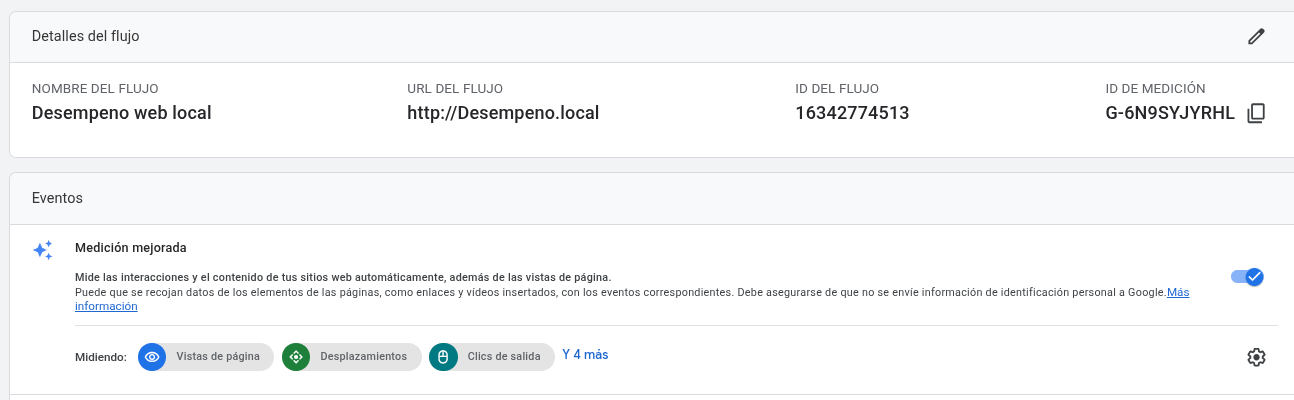
\includegraphics[width=\linewidth]{FLujo de datos.png}\caption{Flujo de datos}\end{subfigure}
\begin{subfigure}{0.49\textwidth}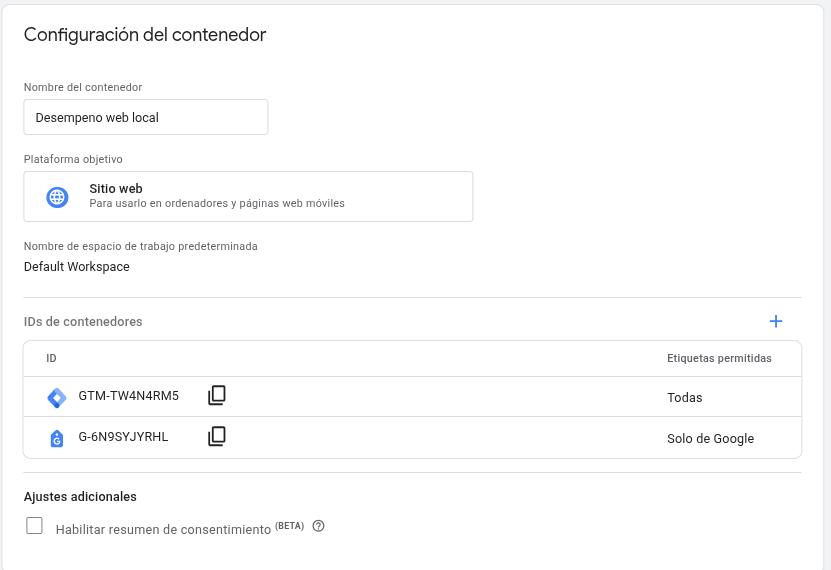
\includegraphics[width=\linewidth]{Contenedor.png}\caption{Contenedor de Tag Manager}\end{subfigure}\\[4pt]
\begin{subfigure}{0.49\textwidth}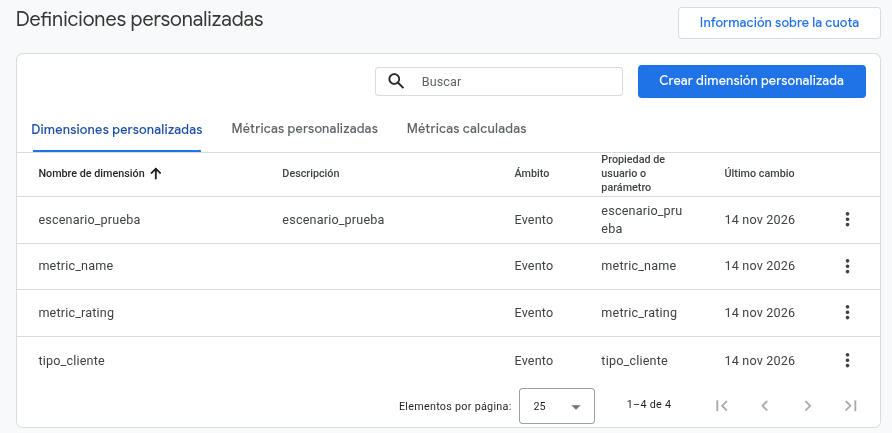
\includegraphics[width=\linewidth]{Dimensiones person.png}\caption{Dimensiones personalizadas}\end{subfigure}
\begin{subfigure}{0.49\textwidth}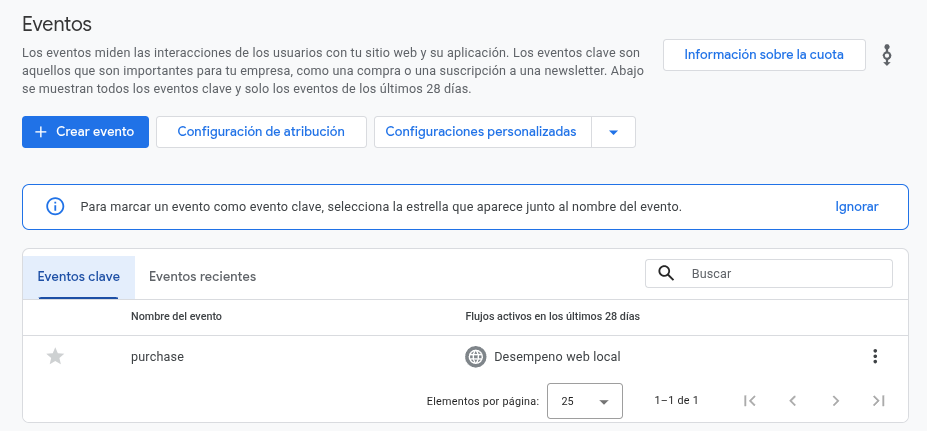
\includegraphics[width=\linewidth]{Eventos clave.png}\caption{\codigo{purchase} como evento clave}\end{subfigure}
\caption{Configuración de GA4.}
\end{figure}

\begin{figure}[H]
\centering
\begin{subfigure}{0.42\textwidth}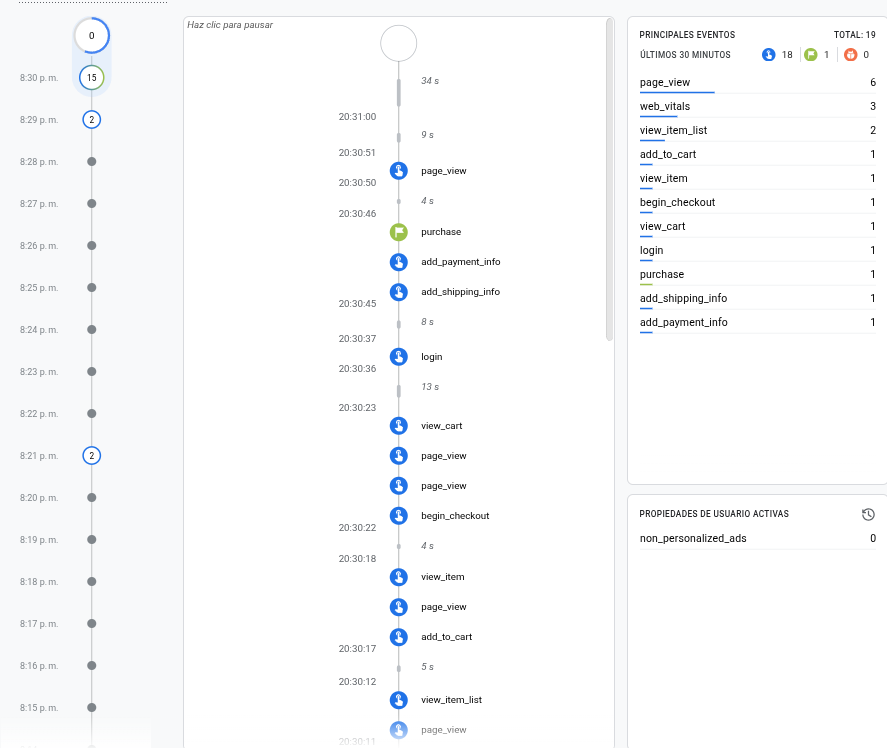
\includegraphics[width=\linewidth]{DebugView.png}\caption{DebugView de una compra}\end{subfigure}
\begin{subfigure}{0.56\textwidth}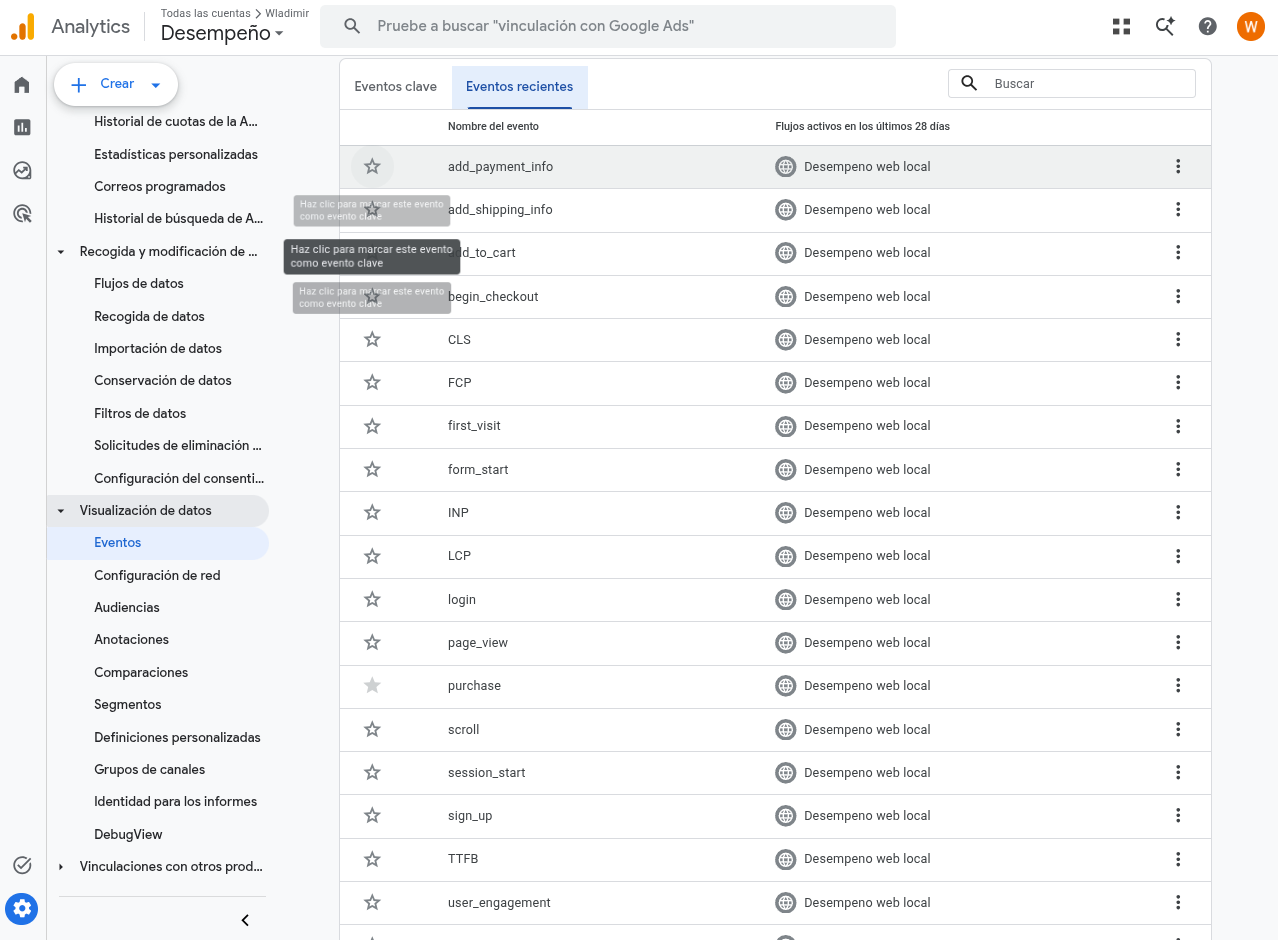
\includegraphics[width=\linewidth]{Eventos.png}\caption{Eventos recibidos}\end{subfigure}
\caption{Eventos de comercio electrónico en GA4.}
\end{figure}

\subsection{Web Vitals}
La biblioteca \codigo{web-vitals} reporta TTFB, FCP, LCP, INP y CLS a GA4 y,
como respaldo, a \codigo{/api/vitals} (Prometheus). Bajo carga, además, k6 corre
un navegador Chrome real en paralelo (módulo \codigo{k6/browser}) que recorre
home $\rightarrow$ catálogo $\rightarrow$ producto $\rightarrow$ agregar
$\rightarrow$ carrito y registra las Web Vitals de cada página.

\subsection{Prometheus y Grafana}
Prometheus recolecta cada 5~s la API (latencia por ruta con histogramas, pool de
conexiones, event loop, duración de argon2, compras), la VM (node-exporter), los
contenedores (cAdvisor) y PostgreSQL (postgres-exporter con
\codigo{pg\_stat\_statements}). Para no depender de capturas de pantalla, al
terminar cada prueba un script exporta estas series a CSV
(\codigo{*.servidor.csv}, \codigo{*.rutas.csv}, \codigo{*.consultas.csv}) junto a
los resultados de k6.

% -----------------------------------------------------------------------------
\section{Metodología de pruebas}

\subsection{Perfiles de usuario}
\begin{table}[H]
\centering\small
\begin{tabularx}{\textwidth}{@{}lrX@{}}
\toprule
Perfil & Peso & Recorrido (con pausas de 1--6~s entre pasos) \\
\midrule
Navegante & 50~\% & Home $\rightarrow$ listado $\rightarrow$ 1 a 3 detalles \\
Buscador & 25~\% & Home $\rightarrow$ búsqueda por término $\rightarrow$ búsqueda con un filtro (categoría, precio, orden o stock) $\rightarrow$ detalle \\
Abandono & 15~\% & Detalle $\rightarrow$ agrega al carrito $\rightarrow$ ve el carrito y se va \\
Comprador & 10~\% & Login $\rightarrow$ detalle $\rightarrow$ agrega al carrito $\rightarrow$ checkout (pago simulado) $\rightarrow$ ve la orden \\
\bottomrule
\end{tabularx}
\caption{Perfiles del generador (\codigo{carga/k6/escenarios.js}).}
\end{table}

\subsection{Escenarios y parámetros}
\begin{table}[H]
\centering\small
\begin{tabularx}{\textwidth}{@{}lX@{}}
\toprule
Escenario & Parámetros \\
\midrule
Baja & Modelo cerrado: 5 VUs (subida 1~min, meseta 5~min, bajada 1~min). \\
Normal & Modelo cerrado: 30 VUs (subida 2~min, meseta 10~min, bajada 2~min). \\
Estrés & Modelo abierto (tasa de llegada): mesetas de 10, 20, 30, 40, 50 y 60~sesiones/s de 2~min, subidas de 30~s; pausas $\times$0,25 (\codigo{FACTOR\_PAUSAS}); máximo 1\,000 VUs. \\
\bottomrule
\end{tabularx}
\caption{Escenarios. Todos con 1~min de calentamiento excluido del análisis.}
\end{table}

Baja y normal usan un \emph{modelo cerrado} (un número fijo de usuarios
virtuales), que representa una tienda con una cantidad conocida de visitantes.
El estrés usa un \emph{modelo abierto}: las sesiones llegan a una tasa fija
aunque el servidor se ponga lento, como ocurre con usuarios reales; en un modelo
cerrado la carga bajaría sola al saturarse y ocultaría el problema
(Grafana Labs, s.\,f.).

\subsection{Indicadores y forma de medición}

Se eligieron indicadores que responden tres preguntas: qué tan rápido
responde el sistema, cuánto trabajo alcanza a hacer y qué recurso lo limita.
Se agregaron los de experiencia de usuario que pide la guía.

\begin{table}[H]
\centering\small
\begin{tabularx}{\textwidth}{@{}>{\raggedright\arraybackslash}p{2.9cm}>{\raggedright\arraybackslash}X>{\raggedright\arraybackslash}X@{}}
\toprule
Indicador & Por qué se eligió & Cómo se midió \\
\midrule
Latencia p50, p95 y p99 &
  El promedio oculta a los usuarios que esperan mucho. El p50 es la
  experiencia típica, el p95 la de casi todos y el p99 muestra la cola
  (Dean y Barroso, 2013; Jain, 1991). &
  k6 (\codigo{http\_req\_duration}) por página, con la etiqueta
  \codigo{pagina}; histogramas de prom-client en la API. \\
Throughput (req/s y sesiones/s), ofrecido frente a logrado &
  Mientras el logrado sigue al ofrecido hay capacidad; cuando se separa, el
  sistema está saturado. &
  k6 (\codigo{http\_reqs}, \codigo{iterations}) y tasa de peticiones en
  Prometheus. \\
Tasa de error &
  Un sistema puede ser rápido porque rechaza peticiones. Se separan los
  errores del servidor de los del generador. &
  k6 (\codigo{http\_req\_failed} y \emph{checks}); respuestas 5xx en
  Prometheus. \\
Uso de CPU, memoria, disco y pool de conexiones &
  Identifican el recurso limitante y permiten aplicar la ley de utilización
  (Menascé et al., 2004). &
  node-exporter (VM), cAdvisor (contenedores) y métricas del pool en la
  API, cada 5~s. \\
Consultas SQL más costosas &
  Ubican el cuello de botella dentro de la base de datos. &
  \codigo{pg\_stat\_statements} (PostgreSQL Global Development Group, s.\,f.). \\
Web Vitals p75 (TTFB, LCP, INP, CLS) &
  Miden la experiencia percibida en el navegador; Google usa el p75 y define
  umbrales «bueno» (Walton, 2020). &
  Navegador real de k6 en paralelo y biblioteca \codigo{web-vitals} hacia GA4
  y Prometheus. \\
Rebote, duración, vistas por sesión y conversión &
  Muestran si la carga cambia el comportamiento de los usuarios
  (Google, s.\,f.). &
  GA4 segmentado por \codigo{escenario\_prueba}; conversión = compras
  correctas / sesiones de k6. \\
\bottomrule
\end{tabularx}
\caption{Indicadores escogidos, su justificación y su forma de medición.}
\end{table}

Para que las mediciones sean comparables, cada escenario se ejecutó tres veces,
se excluyó el minuto de calentamiento y se reporta el promedio con el mínimo y
el máximo. Cada conclusión se contrastó con dos fuentes, el cliente (k6) y el
servidor (Prometheus), porque una sola puede engañar (sección~\ref{sec:limitaciones}).

\paragraph{Umbrales (SLO).} Definidos antes de ejecutar las pruebas
(Beyer et al., 2016): errores~<~1~\%, p95~<~800~ms, p99~<~1\,500~ms,
p95 del detalle~<~1\,000~ms, checkout completo p95~<~2\,000~ms y checks~>~99~\%.

\paragraph{Calibración.} Una prueba piloto (10 VUs) estimó con la ley de
utilización ($U = X \cdot S$) (Menascé et al., 2004) una capacidad de $\sim$22~sesiones/s; tras la carga
normal la estimación subió a $\sim$37~sesiones/s y con ella se fijaron los
escalones del estrés (10--60).

\paragraph{Entorno del generador.} PC con 6 CPU y 23~GiB de RAM, k6~v2.4.0, red
doméstica por cable (Ethernet), con Docker local detenido durante las pruebas.
Se registró la CPU del generador en cada ejecución para descartar que fuera el
cuello de botella.

\paragraph{Protocolo.} Cada ejecución (\codigo{carga/ejecutar.sh}) guarda los
metadatos (commit, hora de inicio y fin, parámetros), el reporte HTML y el
resumen JSON de k6, el CSV crudo, las Web Vitals del navegador real, la CPU del
generador y las métricas del servidor exportadas desde Prometheus. Se hicieron
\textbf{tres repeticiones} de cada escenario; los resultados se reportan como
promedio [mínimo--máximo]. La bitácora (\codigo{carga/bitacora.md}) registra las
11 ejecuciones, incluida una de estrés invalidada (sección~\ref{sec:limitaciones}).

% -----------------------------------------------------------------------------
\section{Resultados}

\subsection{Carga baja y normal}

\begin{table}[H]
\centering\small
\begin{tabular}{@{}lrr@{}}
\toprule
Indicador & Baja (5 VUs) & Normal (30 VUs) \\
\midrule
Promedio (ms)      & 12,0 [11,8--12,2] & 11,8 [11,4--12,0] \\
Mediana (ms)       & 8,9 [8,7--9,0]    & 8,5 [8,5--8,6] \\
p90 (ms)           & 13,9 [13,6--14,4] & 12,6 [12,4--12,8] \\
p95 (ms)           & 18,5 [17,5--20,0] & 17,5 [16,9--18,1] \\
p99 (ms)           & 117,5 [116,8--118,7] & 121,8 [120,4--122,8] \\
Throughput (req/s) & 1,41 [1,40--1,42] & 8,42 [8,38--8,49] \\
Sesiones/s         & 0,356 [0,349--0,363] & 2,137 [2,119--2,159] \\
Tasa de error (\%) & 0,00 & 0,00 \\
Compras exitosas   & 17 [15--18] & 184 [172--193] \\
\bottomrule
\end{tabular}
\caption{Indicadores globales (promedio [mín--máx] de 3 repeticiones, fase de medición).}
\label{tab:baja-normal}
\end{table}

Con seis veces más carga, la latencia no cambia: el sistema trabaja lejos de su
capacidad (CPU de la VM $\approx$~6~\% en baja y 11~\% en normal). El p99 de
$\sim$120~ms corresponde al \emph{login}, que es lento por diseño (argon2id). La
ley de Little (Little, 1961) se cumple: en normal, $N = X\,(R+Z) = 2{,}663 \times 11{,}32
\approx 30$~VUs.

\begin{table}[H]
\centering\small
\begin{tabular}{@{}lrrrrr@{}}
\toprule
Página & Mediana & p90 & p95 & p99 & n por repetición \\
\midrule
Home      & 5,6 & 7,3 & 8,6 & 20,4 & $\sim$1\,450 \\
Listado   & 6,4 & 8,1 & 9,7 & 23,6 & $\sim$950 \\
Búsqueda  & 7,7 & 10,1 & 12,3 & 31,4 & $\sim$990 \\
Detalle   & 9,6 & 12,9 & 15,6 & 29,2 & $\sim$2\,880 \\
Carrito   & 9,8 & 12,8 & 14,7 & 22,3 & $\sim$780 \\
Login     & 119,5 & 150,2 & 175,5 & 216,8 & $\sim$180 \\
Checkout  & 12,6 & 18,0 & 20,3 & 27,2 & $\sim$180 \\
Orden     & 6,1 & 7,1 & 8,2 & 10,9 & $\sim$180 \\
\bottomrule
\end{tabular}
\caption{Latencia por página con carga normal (ms, promedio de 3 repeticiones).}
\end{table}

\begin{figure}[H]
\centering
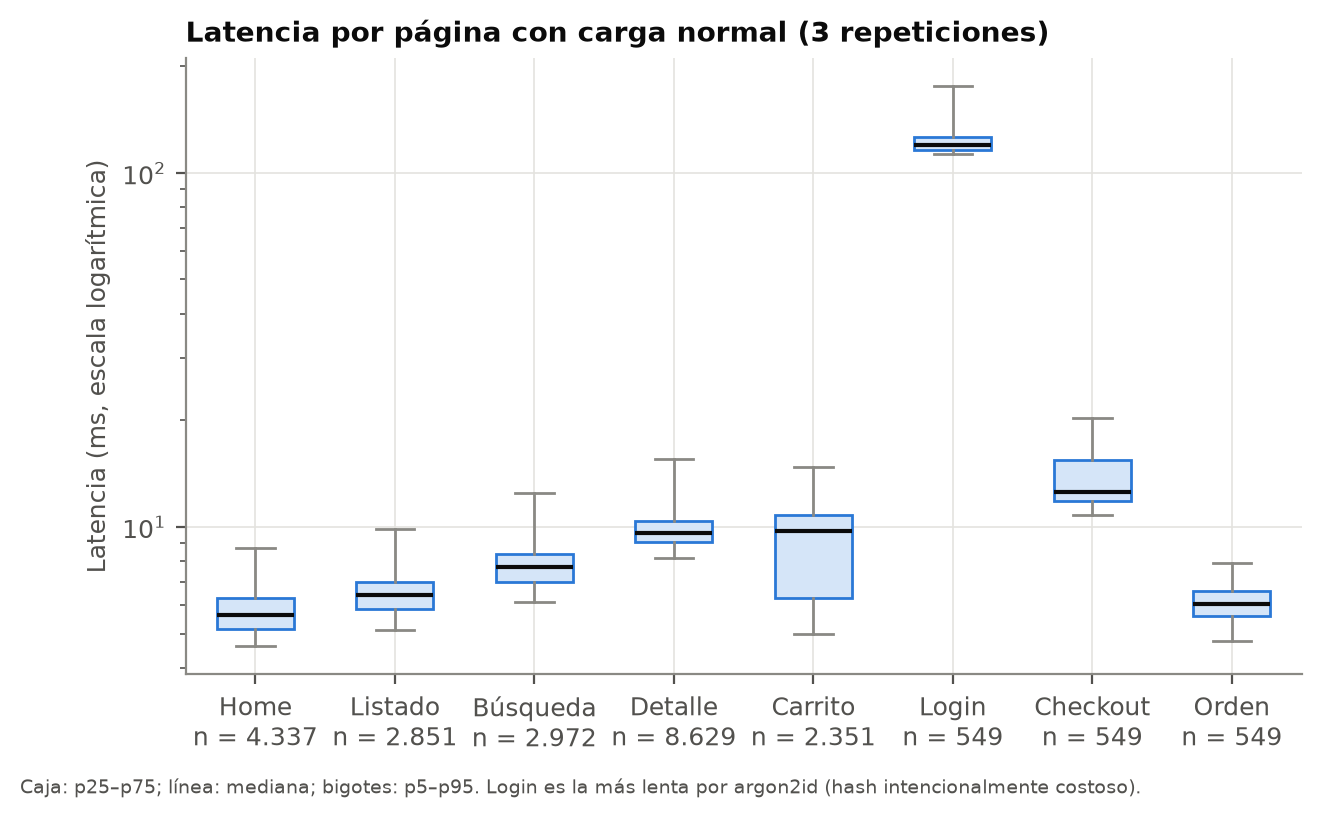
\includegraphics[width=0.85\textwidth]{08_boxplot_paginas_normal.png}
\caption{Distribución de la latencia por página con carga normal. Las páginas con
más datos (detalle, búsqueda) son más lentas que la home; el login domina por argon2id.}
\end{figure}

\begin{figure}[H]
\centering
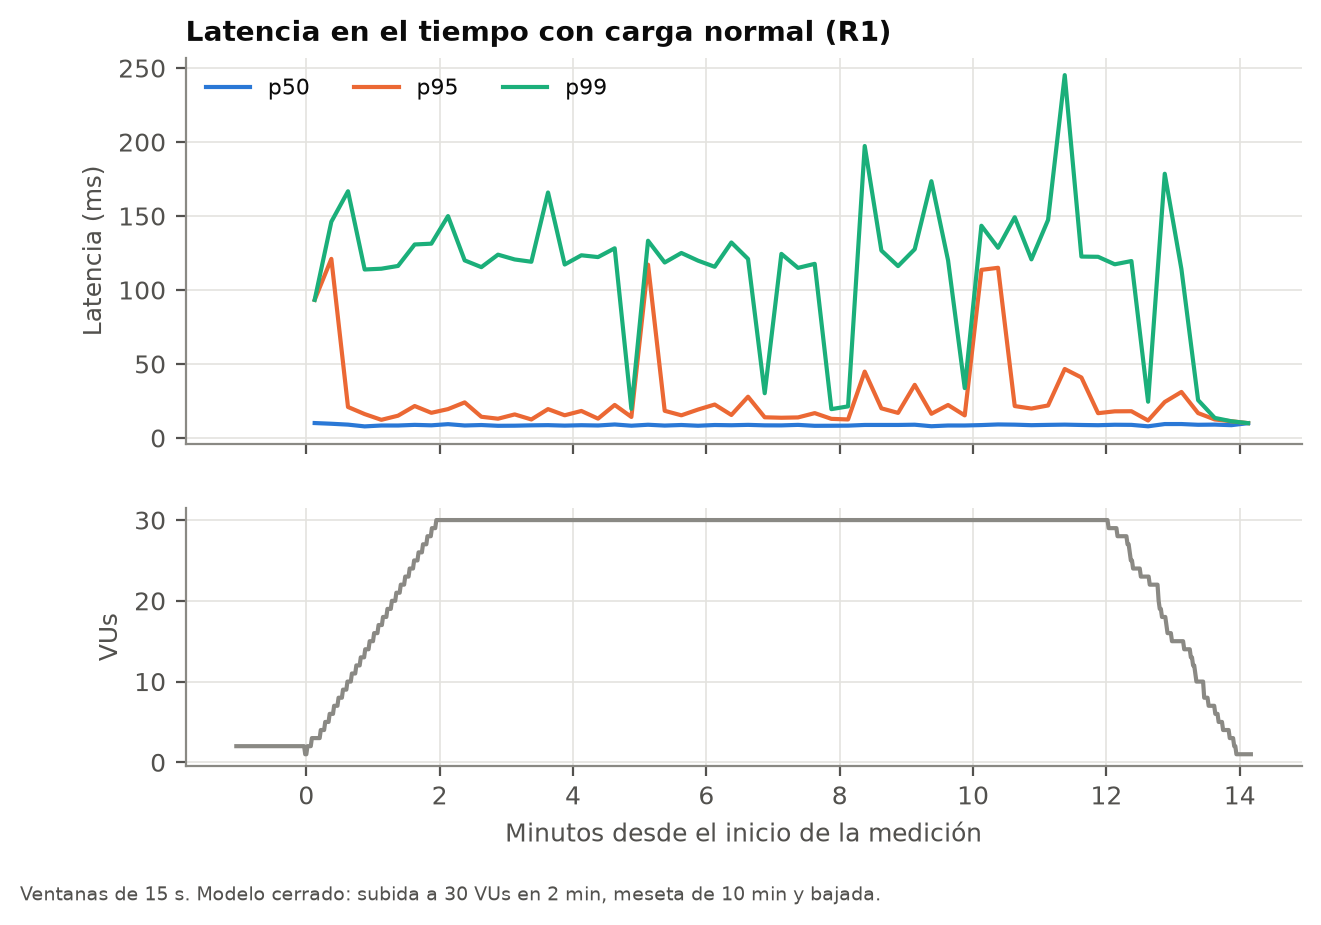
\includegraphics[width=0.85\textwidth]{02_latencia_tiempo_normal.png}
\caption{Latencia en el tiempo con carga normal: estable durante toda la meseta.}
\end{figure}

\subsection{Estrés escalonado}

\begin{figure}[H]
\centering
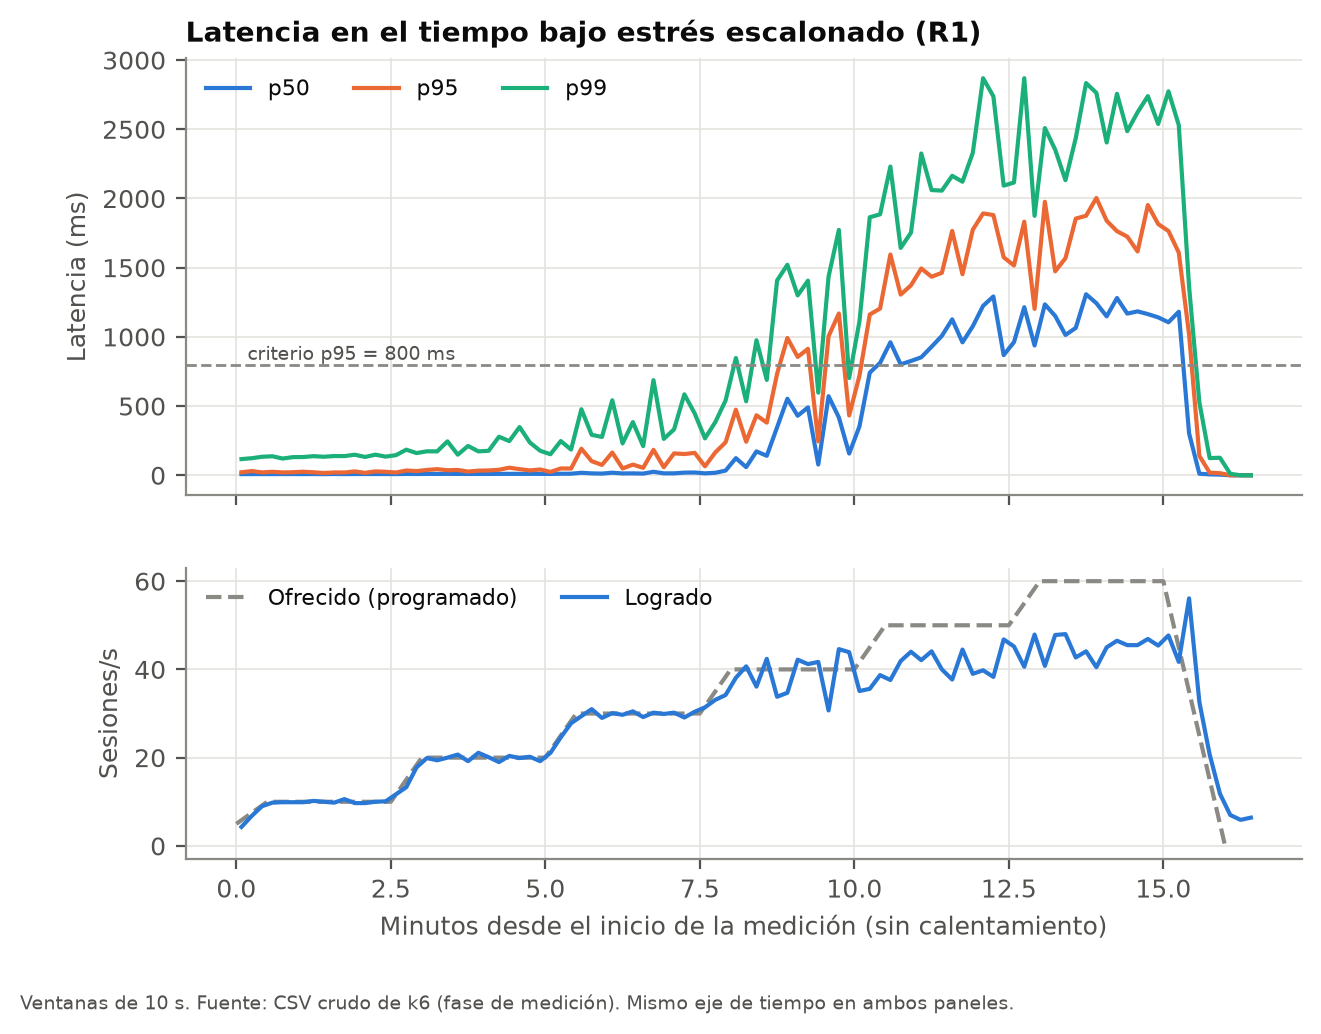
\includegraphics[width=0.9\textwidth]{01_latencia_tiempo_estres.png}
\caption{Latencia en el tiempo y tasa de sesiones ofrecida/lograda (estrés, R1).
Desde la meseta de 40~sesiones/s la latencia se dispara y el logrado se separa
de lo ofrecido.}
\end{figure}

\begin{figure}[H]
\centering
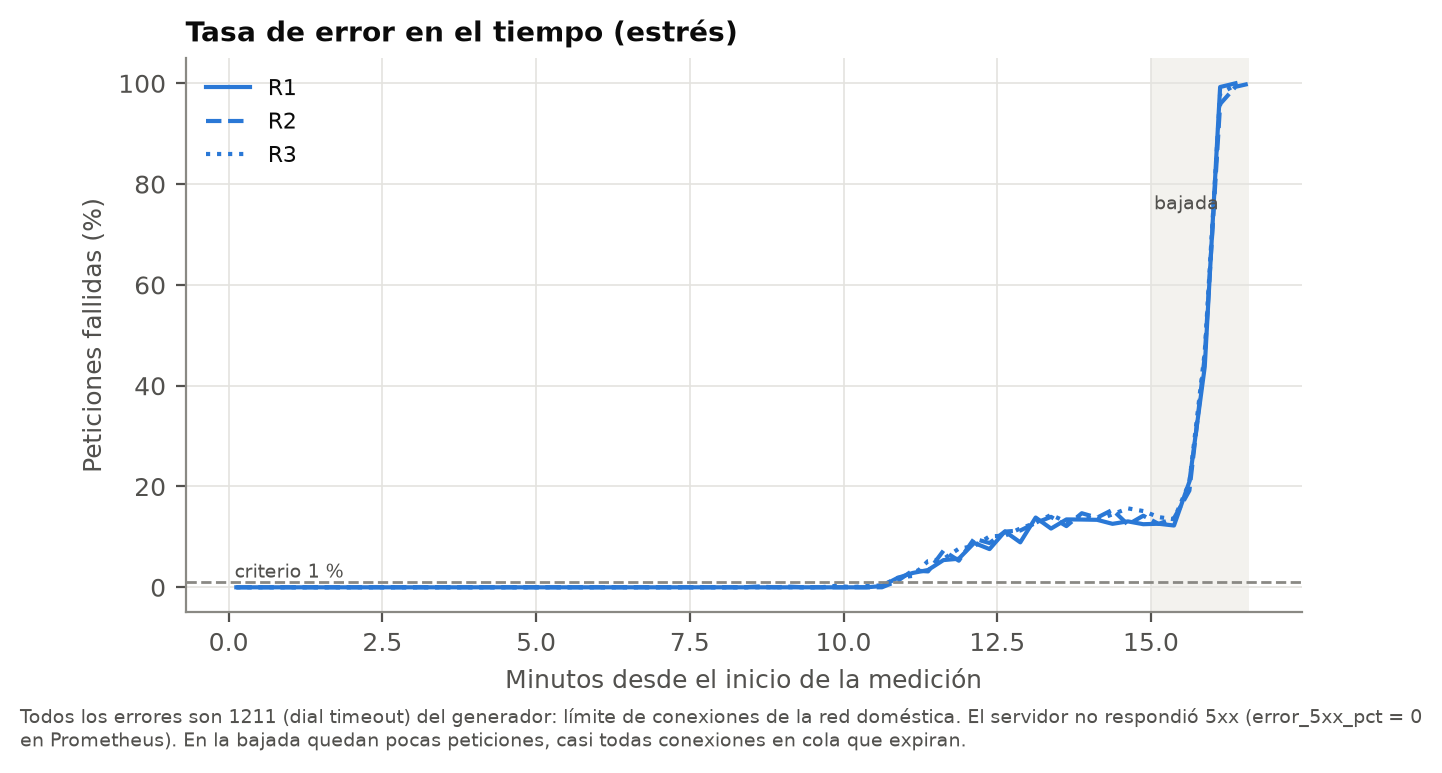
\includegraphics[width=0.85\textwidth]{05_errores_tiempo_estres.png}
\caption{Tasa de error en el tiempo (estrés). Los errores son del generador, no del servidor.}
\end{figure}

\begin{figure}[H]
\centering
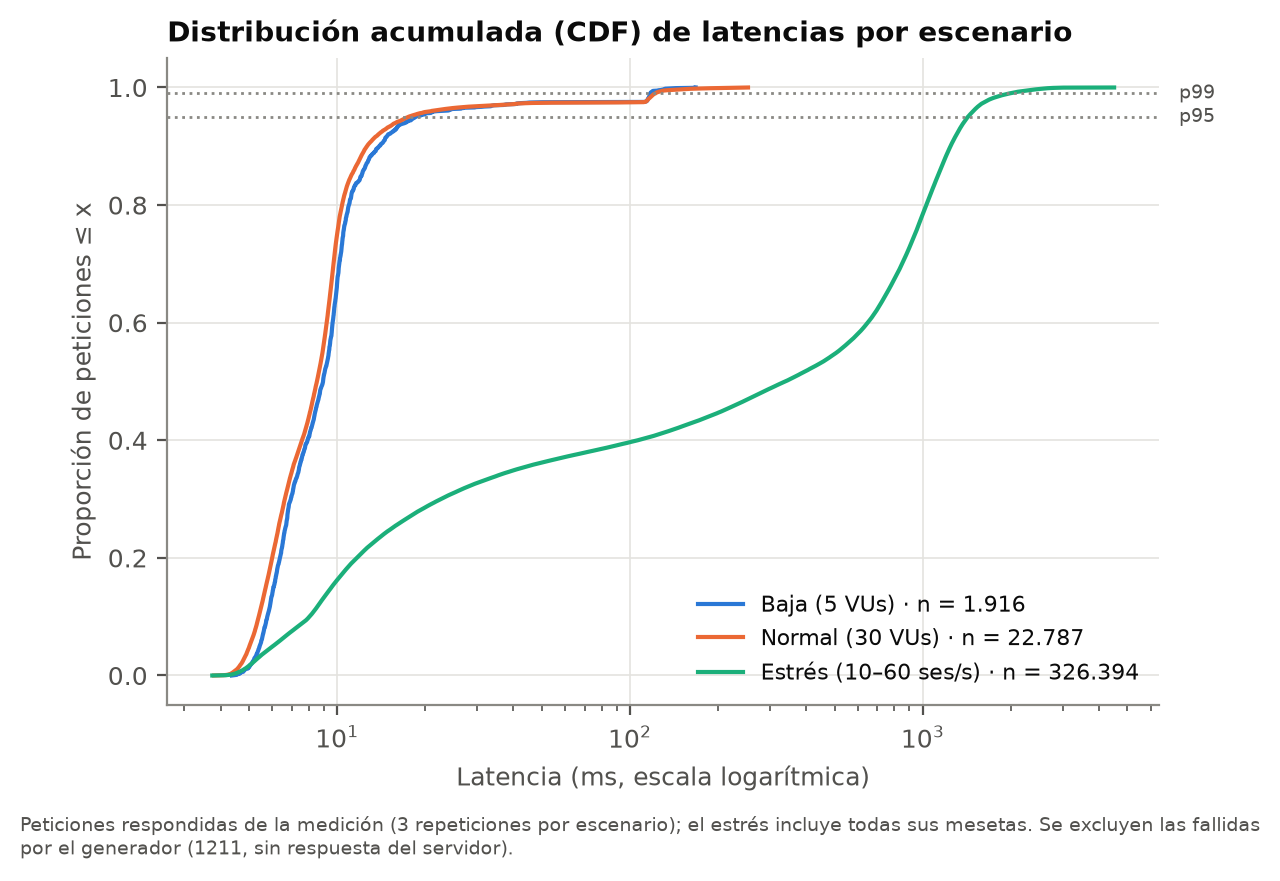
\includegraphics[width=0.85\textwidth]{07_cdf_latencias.png}
\caption{CDF de latencias por escenario. Baja y normal son prácticamente iguales;
el estrés desplaza la cola hasta 1--3~s.}
\end{figure}

\subsection{Recursos del servidor}

\begin{figure}[H]
\centering
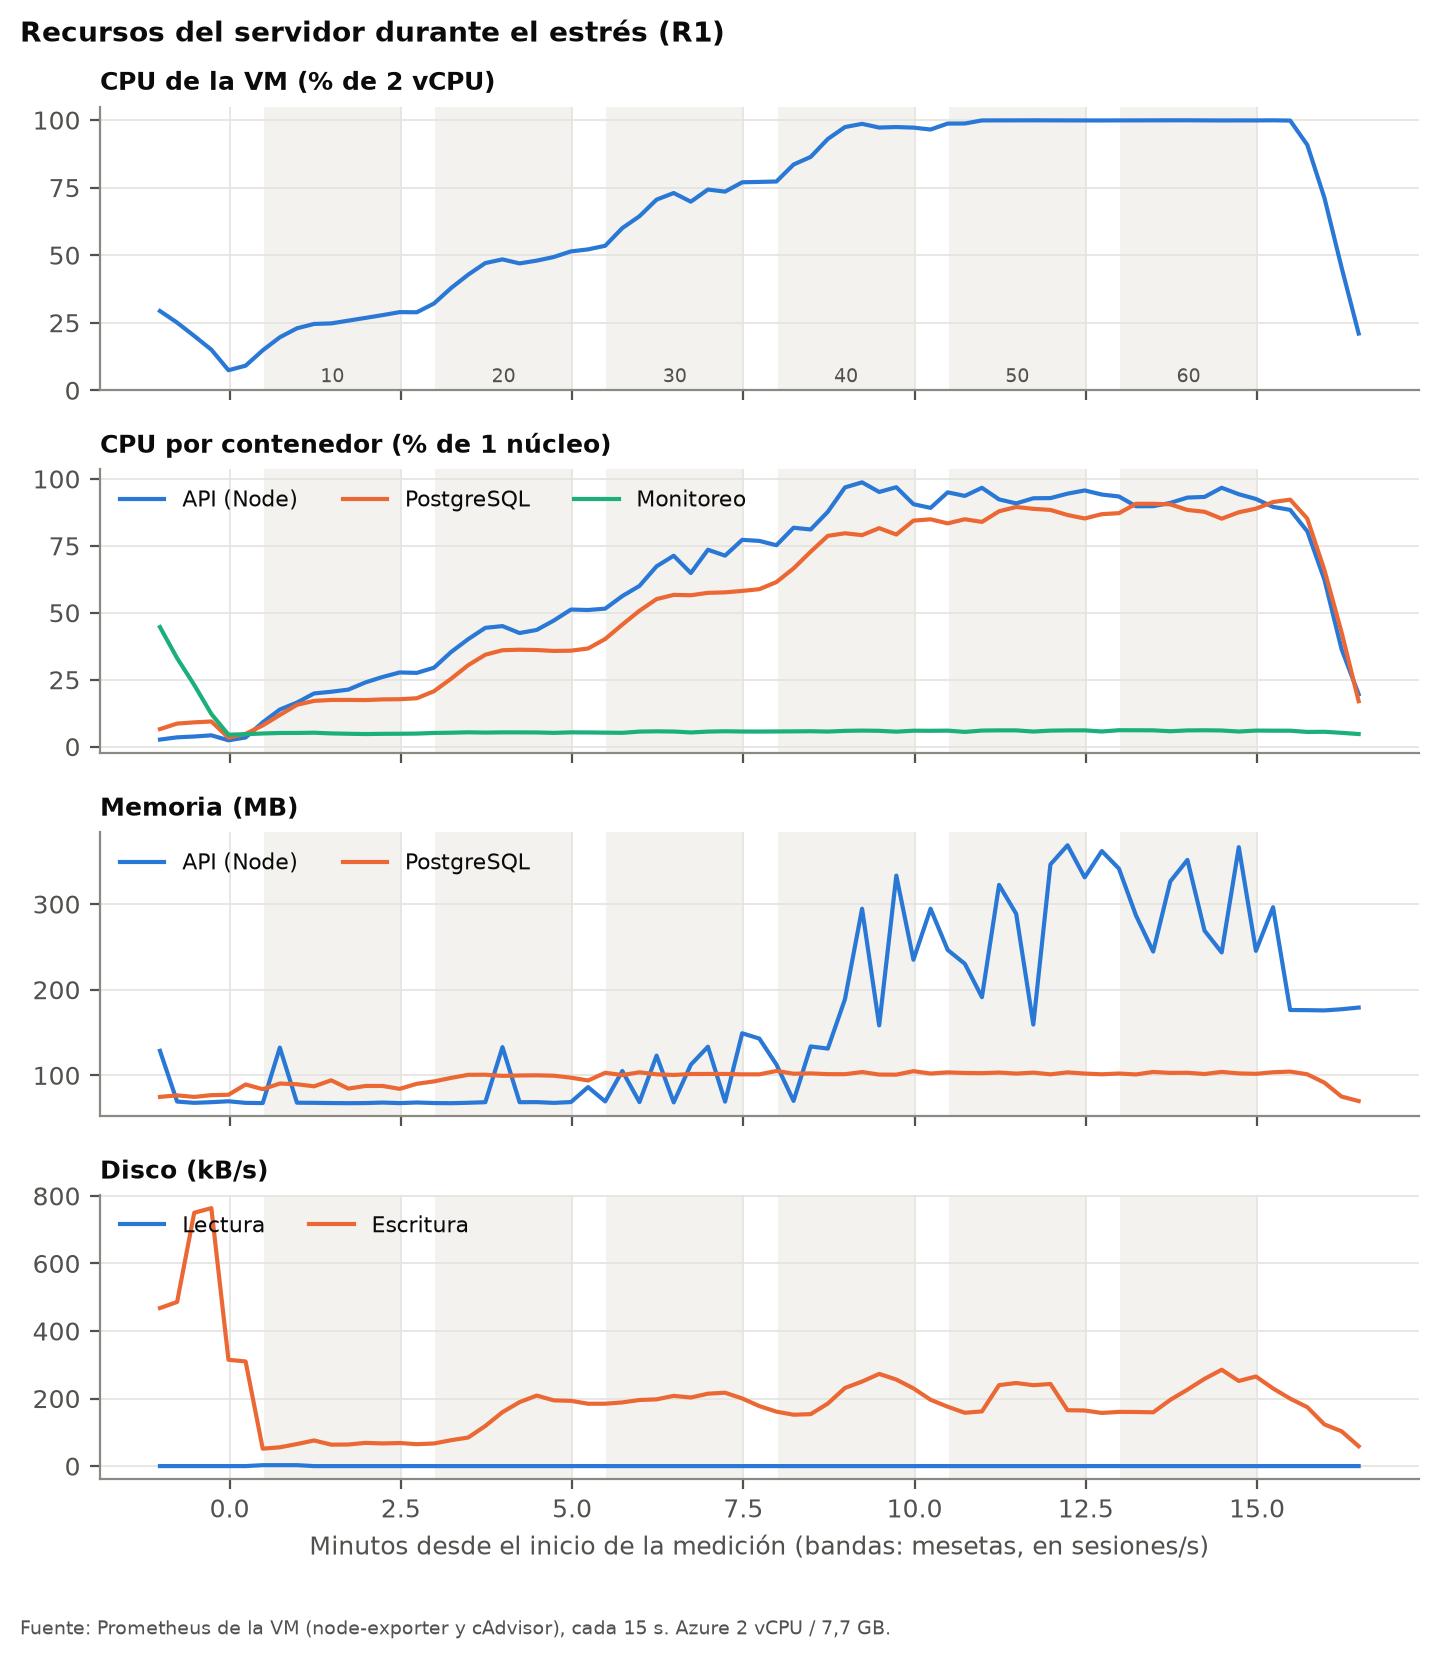
\includegraphics[width=0.9\textwidth]{06_recursos_servidor_estres.png}
\caption{CPU, memoria y disco del servidor durante el estrés (R1), en la misma
escala temporal. La CPU de la VM llega al 95~\% en la meseta de 40 y al 100~\% desde 50;
memoria y disco no se acercan a sus límites.}
\end{figure}

% -----------------------------------------------------------------------------
\section{Punto de saturación y recurso limitante}

\begin{table}[H]
\centering\scriptsize
\setlength{\tabcolsep}{4pt}
\begin{tabular}{@{}rrrrrrrrl@{}}
\toprule
Ofrecido & Logrado & Logrado & p50 & p95 & p99 & Error & CPU VM & CPU api / db \\
(ses/s) & (ses/s) & (req/s) & (ms) & (ms) & (ms) & (\%)* & (\%) & (\% de 1 núcleo) \\
\midrule
10 & 10,0 & 39,7  & 9    & 23   & 139  & 0,0  & 26  & 23 / 17 \\
20 & 20,0 & 78,8  & 10   & 36   & 195  & 0,0  & 47  & 44 / 35 \\
30 & 29,9 & 118,6 & 15   & 117  & 346  & 0,0  & 72  & 68 / 55 \\
40 & 39,5 & 155,5 & 242  & 705  & 1\,110 & 0,0  & 95  & 92 / 79 \\
50 & 40,4 & 164,4 & 900  & 1\,507 & 2\,090 & 5,8  & 100 & 94 / 86 \\
60 & 44,1 & 171,6 & 1\,077 & 1\,803 & 2\,480 & 13,7 & 100 & 94 / 86 \\
\bottomrule
\end{tabular}
\caption{Estrés por meseta (promedio de R1--R3; últimos 100~s de cada meseta).
* Errores 1211 del generador. Detalle con mínimos y máximos en
\codigo{carga/resultados/ESTRES/RESUMEN.md}.}
\label{tab:saturacion}
\end{table}

\begin{figure}[H]
\centering
\begin{subfigure}{0.49\textwidth}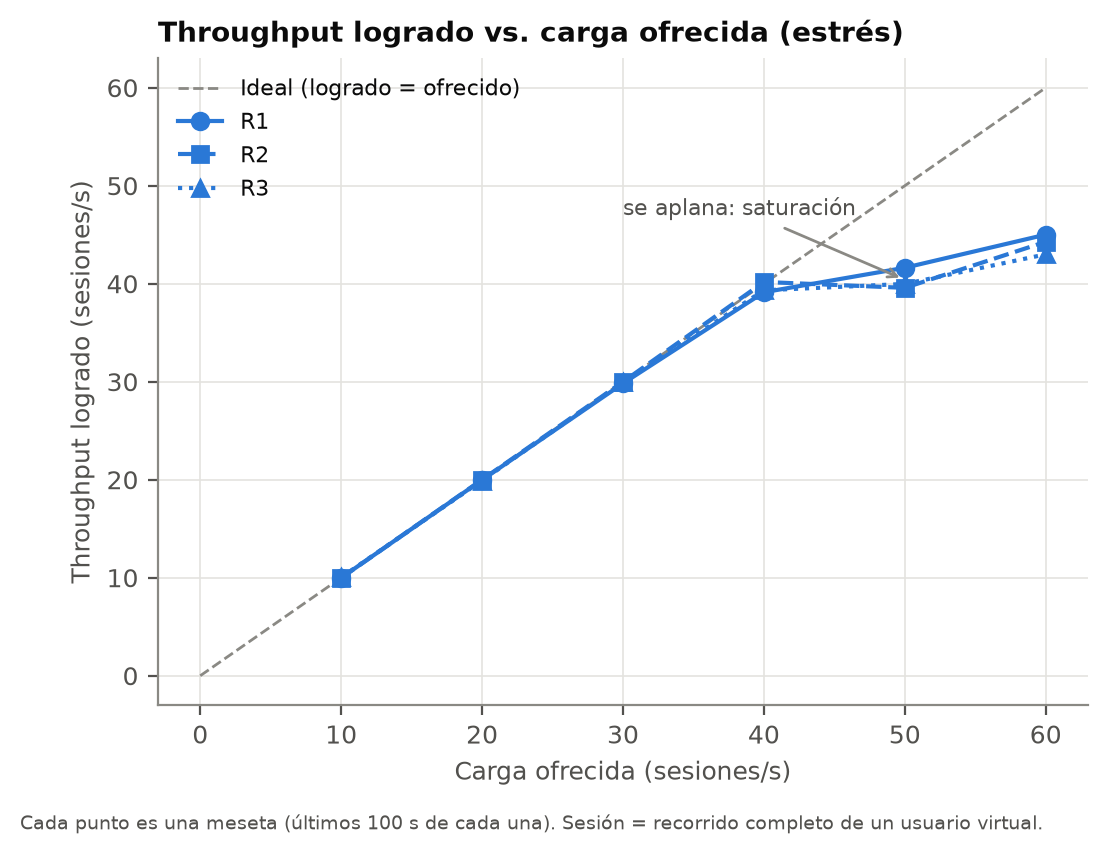
\includegraphics[width=\linewidth]{03_throughput_vs_ofrecido.png}\caption{Throughput logrado vs. ofrecido}\end{subfigure}
\begin{subfigure}{0.49\textwidth}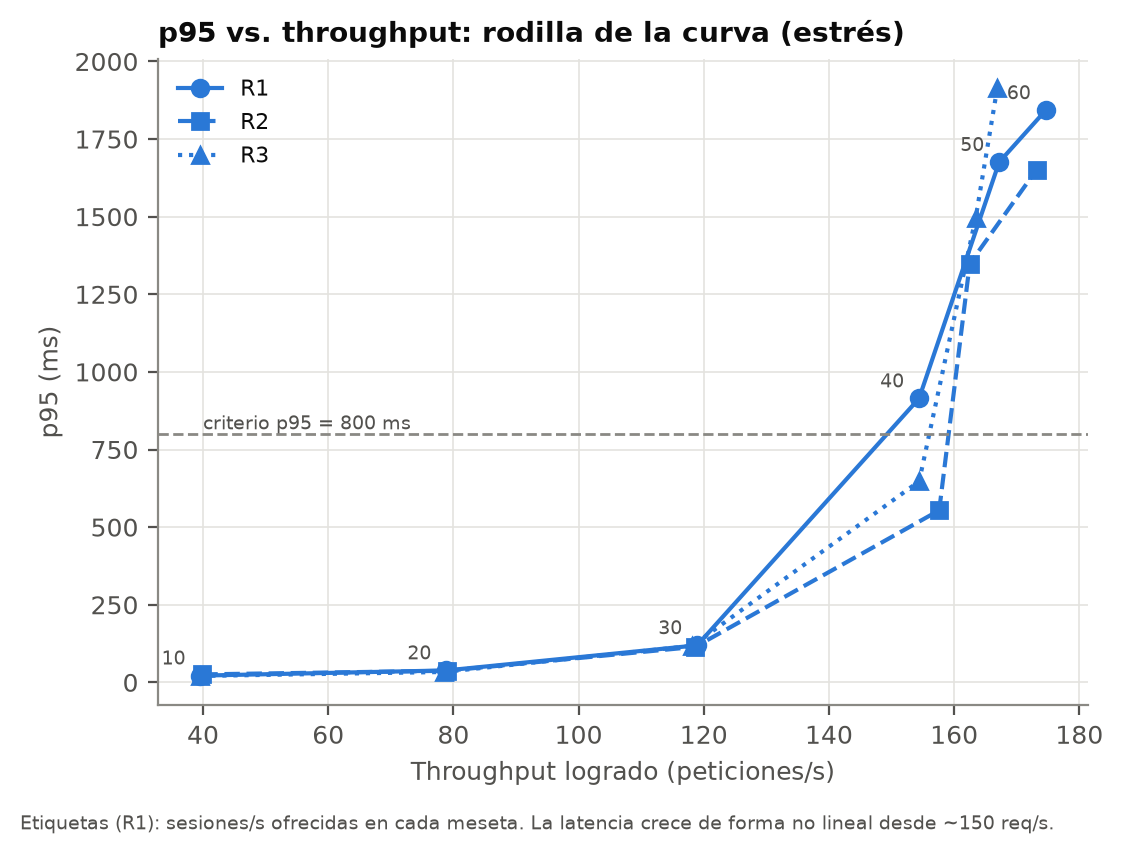
\includegraphics[width=\linewidth]{04_p95_vs_throughput.png}\caption{p95 vs. throughput}\end{subfigure}
\caption{Identificación del punto de saturación (guía, sección 6.5).}
\end{figure}

\begin{clave}[Punto de saturación y recurso limitante]
\begin{itemize}
  \item \textbf{Rodilla:} 40~sesiones/s ($\sim$155~req/s). La CPU de la VM pasa
        al 95~\% y el p95 salta de 117~ms a 705~ms [554--914].
  \item \textbf{Punto de saturación} (primera meseta con p95~>~800~ms, error~>~1~\%
        o logrado~<~90~\% de lo ofrecido): 50~sesiones/s en R2 y R3; en R1 ya en
        40 (p95 914~ms).
  \item \textbf{Throughput máximo:} $\sim$172~req/s ($\sim$44~sesiones/s) con la
        CPU al 100~\%.
  \item \textbf{Recurso limitante: CPU de la VM} (2 vCPU), compartida por la API
        ($\sim$94~\% de un núcleo) y PostgreSQL ($\sim$86~\%). Las conexiones en
        espera del pool (155--343) son consecuencia: PostgreSQL responde más
        lento sin CPU libre. Memoria, disco y red no se saturan.
  \item \textbf{Validación analítica:} a 30~sesiones/s la VM usa el 72~\% de 2
        núcleos, es decir $S \approx 2 \times 0{,}72 / 30 \approx 48$~ms de CPU
        por sesión, y $X_{\max} \approx 2 / 0{,}048 \approx 41$~sesiones/s;
        lo medido fue 40--45.
\end{itemize}
\end{clave}

% -----------------------------------------------------------------------------
\section{Experiencia de usuario: sin carga vs.\ bajo carga}

\begin{figure}[H]
\centering
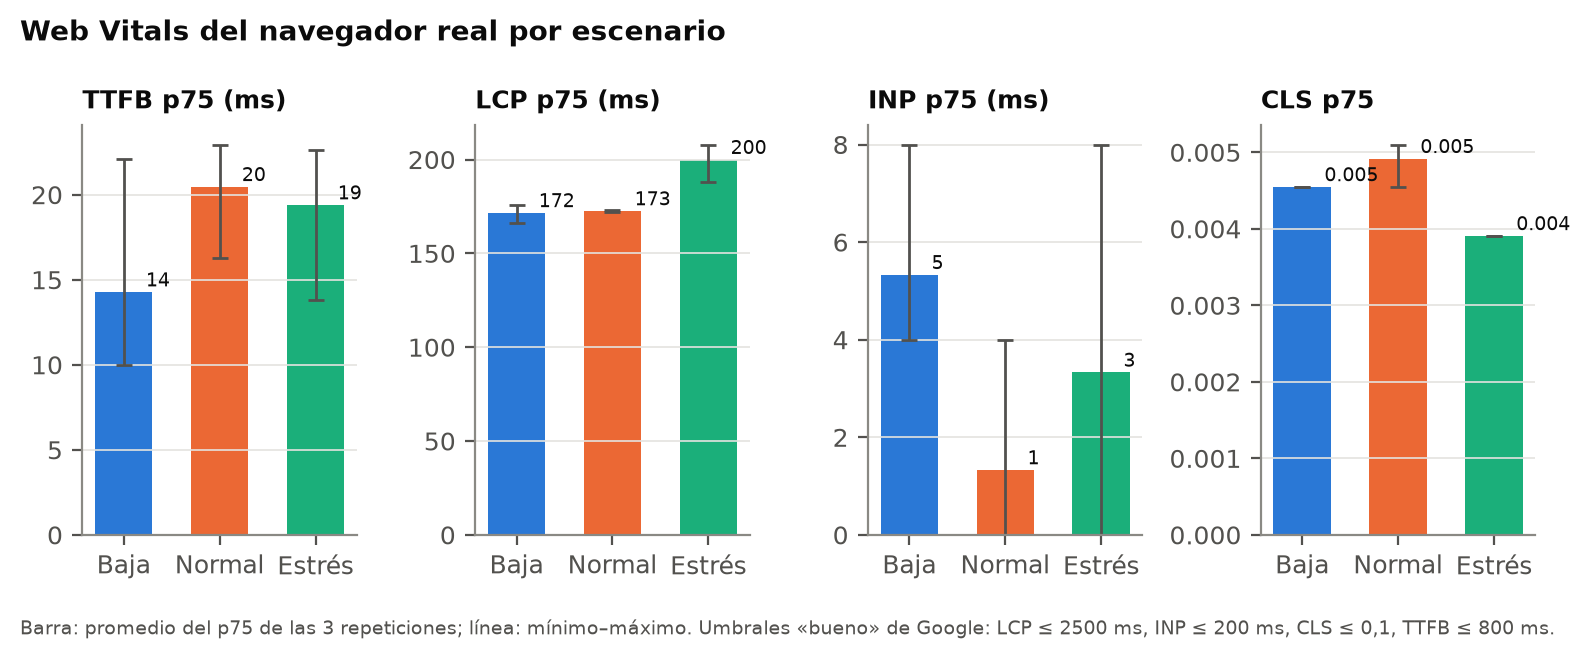
\includegraphics[width=\textwidth]{09_web_vitals_escenarios.png}
\caption{Web Vitals p75 del navegador real en cada escenario.}
\end{figure}

\begin{table}[H]
\centering\small
\resizebox{\textwidth}{!}{%
\begin{tabular}{@{}lrrrr@{}}
\toprule
Indicador & Sin carga (real) & Carga baja & Carga normal & Estrés \\
\midrule
TTFB p75 (ms) & -- & 14 [10--22] & 20 [16--23] & 19 [14--23] \\
LCP p75 (s)   & -- & 0,172 [0,166--0,176] & 0,173 [0,172--0,173] & 0,200 [0,188--0,208] \\
INP p75 (ms)  & -- & 5 [4--8] & 1 [0--4] & 3 [0--8] \\
CLS p75       & -- & 0,005 & 0,005 & 0,004 \\
\midrule
Sesiones GA4                       & 17      & 98  & 186 & 159 \\
Tasa de rebote GA4 (\%)            & 23,53   & 0   & 0   & 1,26 \\
Tasa de interacción GA4 (\%)       & 76,47   & 100 & 100 & 98,74 \\
Duración media de sesión GA4 (s)   & 931     & 14  & 14  & 13 \\
Tiempo de interacción medio (s)    & 114     & 3   & 3   & 3 \\
Vistas por sesión GA4              & 24,65   & 4   & 4   & 4 \\
\midrule
Conversión sesión $\rightarrow$ compra, k6 (\%) & -- & 9,5 [8,7--10,1] & 9,5 [8,9--10,0] & 9,4 [9,4--9,5] \\
\bottomrule
\end{tabular}}
\caption{Indicadores de experiencia de usuario (guía, tabla 6.4). Web Vitals y
conversión: promedio [mín--máx] de 3 repeticiones. GA4: exploración de formato
libre con un segmento por valor de \codigo{escenario\_prueba} (total de las
repeticiones). «Sin carga (real)»: visitas de los integrantes, sin
\codigo{escenario\_prueba}.}
\end{table}

Todas las Web Vitals quedan dentro del rango «bueno» de Google en los tres
escenarios. Como se esperaba, el LCP empeora con el estrés (+16~\%, de 172 a
200~ms) porque depende del servidor, mientras que el CLS no cambia (depende del
diseño). El p75 cambia poco porque las visitas del navegador real se reparten en
todas las mesetas, incluidas las no saturadas; durante la saturación hubo una
navegación cortada a los 30~s y un LCP máximo de 137~s (R1), que el p75 no refleja.

\begin{figure}[H]
\centering
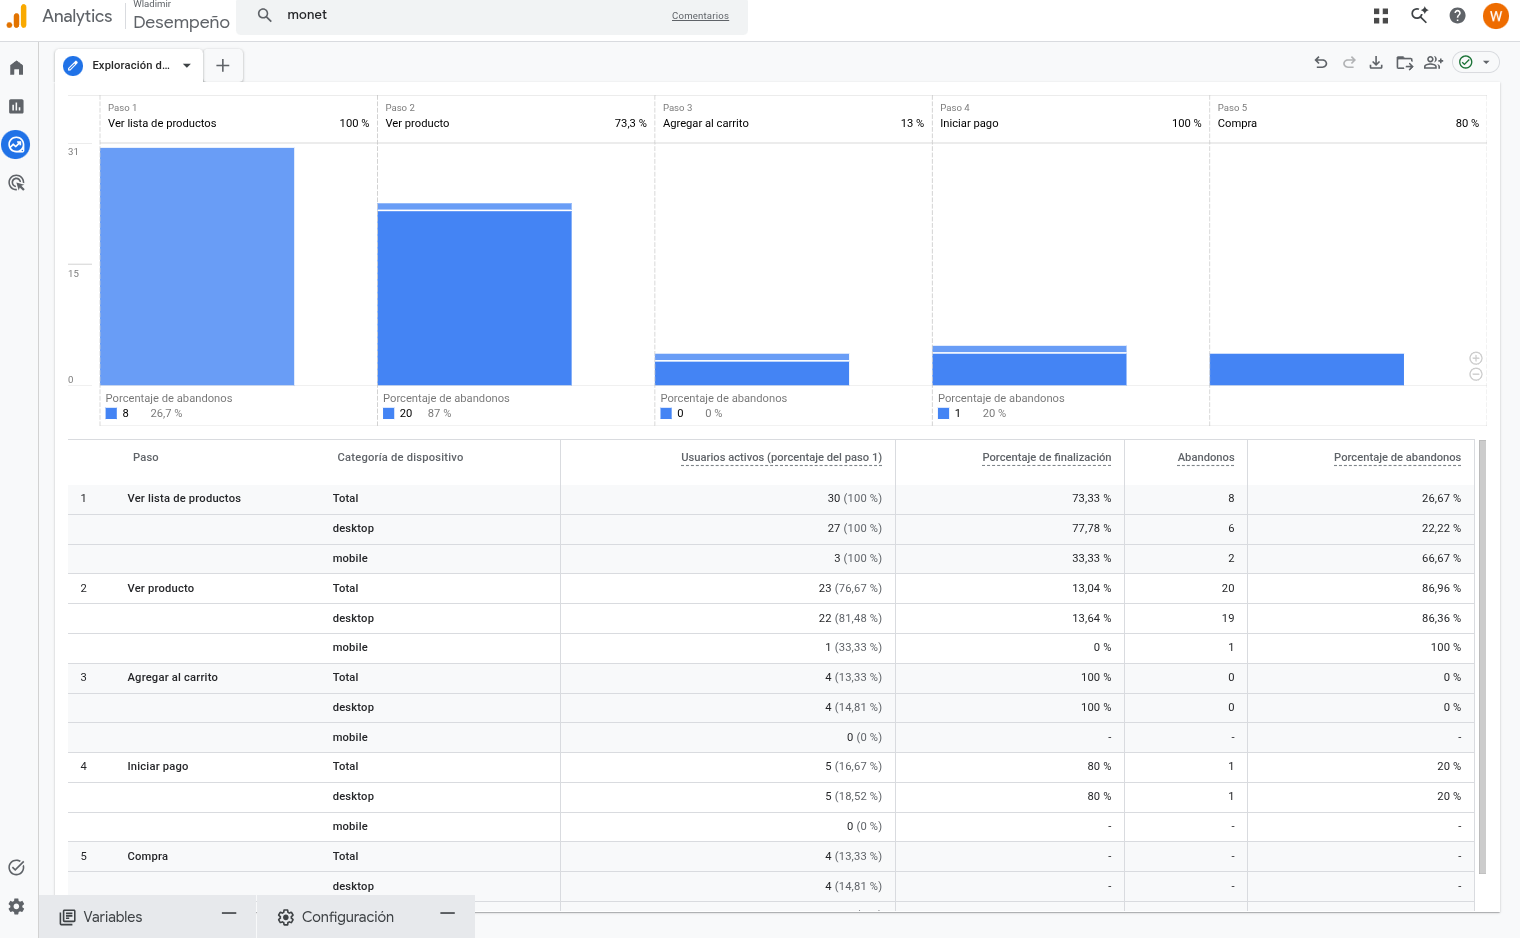
\includegraphics[width=0.9\textwidth]{Embudo.png}
\caption{Embudo de conversión en GA4: lista de productos $\rightarrow$ producto
$\rightarrow$ carrito $\rightarrow$ inicio de pago $\rightarrow$ compra.}
\end{figure}

En GA4 solo aparecen las sesiones del navegador real, porque k6 HTTP no
ejecuta JavaScript. Cada iteración del navegador es una sesión nueva, y los
conteos coinciden con k6: 98 sesiones en carga baja (32 + 32 + 34 iteraciones)
y 186 en carga normal (62 + 61 + 63). En el estrés GA4 registró 159 de las 165
iteraciones (incluye la ejecución invalidada, que usó el mismo
\codigo{escenario\_prueba}); las 6 que faltan serían navegaciones que no
alcanzaron a enviar eventos durante la saturación.

Bajo carga baja y normal ninguna sesión rebotó (100~\% de interacción, 14~s de
duración y 4 vistas por sesión). En el estrés la tasa de rebote sube a 1,26~\%
(2 sesiones sin interacción) y la duración baja a 13~s: aunque las páginas
tardaron más, el navegador automatizado sigue el mismo guion, de modo que un
rebote solo aparece cuando una navegación se corta antes de registrar
interacción, justo lo que se observó en la saturación. El efecto es pequeño
porque estas sesiones se reparten en todas las mesetas, la mayoría no
saturadas.

Las sesiones reales (sin carga) no son comparables en duración ni en vistas:
son 17 sesiones de los integrantes, que recorrieron el sitio y el panel durante
el desarrollo (15~min y 25 vistas por sesión, 23,5~\% de rebote). Sirven como
referencia de un uso humano, no como línea base del guion.

El navegador real no compra, por lo que bajo carga el embudo de GA4 llega hasta
el carrito y la conversión se mide en el servidor (\codigo{compras\_ok} /
sesiones de k6): se mantiene en $\sim$9,5~\% en los tres escenarios, incluso en
el estrés, con 2\,756 compras [2\,743--2\,763] por repetición y sin compras
fallidas por falta de stock. La saturación hace más lentas las compras, pero
no las pierde.

% -----------------------------------------------------------------------------
\section{Cuellos de botella y propuestas de mejora}

\begin{figure}[H]
\centering
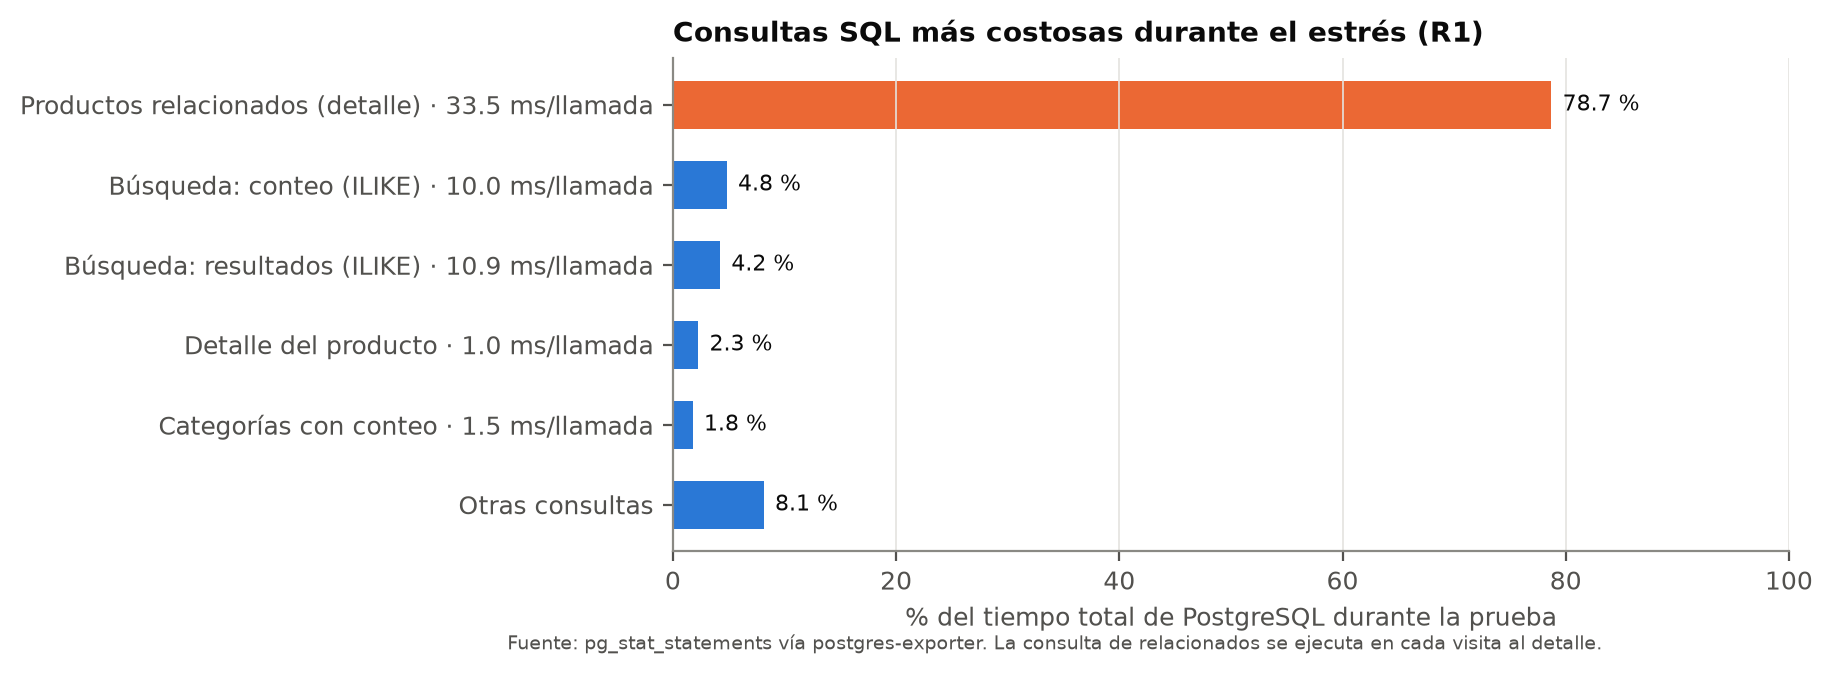
\includegraphics[width=0.9\textwidth]{10_consultas_sql_estres.png}
\caption{Consultas SQL más costosas durante el estrés (\codigo{pg\_stat\_statements}).}
\end{figure}

\begin{enumerate}
  \item \textbf{Productos relacionados (79~\% del tiempo de PostgreSQL).} En cada
        visita al detalle se suman todas las ventas históricas para ordenar los
        relacionados ($\sim$33~ms por llamada bajo estrés). Propuesta: mantener
        las unidades vendidas en una tabla o vista materializada actualizada al
        vender, o guardar el resultado en caché por unos minutos. Se espera
        liberar gran parte de la CPU de PostgreSQL y mover la rodilla hacia
        arriba. Por plazo no se implementó ni se re-midió; queda como la
        primera mejora propuesta.
  \item \textbf{CPU compartida en una VM de 2 vCPU.} Escalar verticalmente (4
        vCPU) o separar PostgreSQL de la API en otra máquina; con la ley de
        utilización, duplicar los núcleos debería acercar la capacidad a
        $\sim$80~sesiones/s.
  \item \textbf{Búsqueda sin índices (\codigo{ILIKE}, $\sim$10~ms por consulta).}
        Un índice trigram (\codigo{pg\_trgm}) sobre nombre y descripción.
  \item \textbf{Login con argon2id} ($\sim$120~ms sin carga, >~1,5~s bajo
        estrés). Es costoso por seguridad; se puede ajustar el costo dentro de
        lo recomendado o limitar los intentos concurrentes.
  \item \textbf{Generador.} Para medir más allá de $\sim$1\,000 conexiones
        simultáneas, ejecutar k6 desde una VM en la nube y no desde una red
        doméstica.
\end{enumerate}

% -----------------------------------------------------------------------------
\section{Limitaciones y amenazas a la validez}
\label{sec:limitaciones}

\begin{itemize}
  \item \textbf{Red del generador.} La primera ejecución de estrés (pausas
        normales, hasta $\sim$400 VUs) fue invalidada: desde $\sim$24~sesiones/s
        k6 no pudo abrir más conexiones (error 1211, \emph{dial timeout}) mientras
        el servidor estaba sano (CPU $\le$~64~\%). Se repitió con pausas
        $\times$0,25, que reduce los VUs necesarios para la misma tasa. Aun así,
        sobre 50~sesiones/s aparecen errores 1211, que no son del servidor.
  \item \textbf{Pausas reducidas en el estrés.} Cambian el tiempo de reflexión de
        las sesiones, no la mezcla de páginas ni la demanda por sesión.
  \item \textbf{Tamaño muestral de GA4.} Solo las sesiones del navegador real
        llegan a GA4 bajo carga (98, 186 y 159 por escenario) y siguen un
        guion fijo, por lo que el rebote y la duración reflejan errores de
        carga y no decisiones de usuarios; además GA4 tarda 24--48~h en
        procesar los datos.
  \item \textbf{Capa gratuita / créditos de estudiante.} Una sola VM de 2 vCPU
        con el monitoreo en la misma máquina ($\sim$4--6~\% de un núcleo).
  \item \textbf{Pago simulado bajo carga.} Por recomendación de la guía, las
        pruebas no cargan el sandbox de Transbank; el flujo de Webpay se validó
        manualmente.
\end{itemize}

% -----------------------------------------------------------------------------
\section{Conclusiones}

\begin{itemize}
  \item El sitio cumple los SLO con holgura en carga baja y normal (p95 $<$
        20~ms, 0~\% errores) y no se degrada al multiplicar la carga por seis.
  \item La capacidad de la configuración actual es de $\sim$40~sesiones/s
        ($\sim$155~req/s); desde ahí la latencia crece de forma no lineal y en 50
        se cruza el criterio de saturación. El máximo es $\sim$172~req/s.
  \item El recurso limitante es la CPU de la VM, y la evidencia apunta a una sola
        consulta (relacionados) como el principal consumidor de la base de
        datos: es la mejora con mejor relación costo/beneficio.
  \item La ley de utilización predijo la capacidad con un error menor al 10~\%,
        lo que valida el modelo y la calibración del estrés.
  \item La experiencia de usuario medida con Web Vitals se mantiene «buena» en
        todos los escenarios en el p75, pero las colas (p99, máximos) muestran
        que bajo saturación algunos usuarios sí esperan varios segundos.
  \item En GA4 el estrés aparece como rebotes (0~\% $\rightarrow$ 1,26~\%) y
        sesiones algo más cortas, y la conversión medida en el servidor se
        mantiene en $\sim$9,5~\%: bajo saturación los usuarios esperan más,
        pero las compras no se pierden.
\end{itemize}

% -----------------------------------------------------------------------------
\section*{Referencias}
\addcontentsline{toc}{section}{Referencias}

\begin{list}{}{\setlength{\leftmargin}{1.5em}\setlength{\itemindent}{-1.5em}
  \setlength{\itemsep}{4pt}\small}
\item Anthropic. (s.\,f.). \emph{Claude Code}. \url{https://www.anthropic.com/claude-code}
\item Beyer, B., Jones, C., Petoff, J. y Murphy, N. R. (Eds.). (2016).
  \emph{Site reliability engineering: How Google runs production systems}. O'Reilly Media.
\item Biryukov, A., Dinu, D. y Khovratovich, D. (2016). Argon2: New generation of
  memory-hard functions for password hashing and other applications. En
  \emph{2016 IEEE European Symposium on Security and Privacy} (pp.~292--302). IEEE.
  \url{https://doi.org/10.1109/EuroSP.2016.31}
\item Dean, J. y Barroso, L. A. (2013). The tail at scale. \emph{Communications
  of the ACM, 56}(2), 74--80. \url{https://doi.org/10.1145/2408776.2408794}
\item Google. (s.\,f.). \emph{Measure ecommerce} [Documentación de Google
  Analytics 4]. \url{https://developers.google.com/analytics/devguides/collection/ga4/ecommerce}
\item Grafana Labs. (s.\,f.). \emph{Open and closed models} [Documentación de
  Grafana k6]. \url{https://grafana.com/docs/k6/latest/using-k6/scenarios/concepts/open-vs-closed/}
\item Jain, R. (1991). \emph{The art of computer systems performance analysis:
  Techniques for experimental design, measurement, simulation, and modeling}. Wiley.
\item Little, J. D. C. (1961). A proof for the queuing formula: $L = \lambda W$.
  \emph{Operations Research, 9}(3), 383--387. \url{https://doi.org/10.1287/opre.9.3.383}
\item Menascé, D. A., Almeida, V. A. F. y Dowdy, L. W. (2004). \emph{Performance
  by design: Computer capacity planning by example}. Prentice Hall.
\item PostgreSQL Global Development Group. (s.\,f.). \emph{pg\_stat\_statements:
  Track statistics of SQL planning and execution} [Documentación de PostgreSQL 16].
  \url{https://www.postgresql.org/docs/16/pgstatstatements.html}
\item Prometheus Authors. (s.\,f.). \emph{Histograms and summaries}
  [Documentación de Prometheus]. \url{https://prometheus.io/docs/practices/histograms/}
\item Transbank. (s.\,f.). \emph{Webpay Plus} [Documentación para
  desarrolladores]. \url{https://www.transbankdevelopers.cl/documentacion/webpay-plus}
\item Walton, P. (2020). \emph{Web Vitals}. web.dev.
  \url{https://web.dev/articles/vitals}
\end{list}

% -----------------------------------------------------------------------------
\section*{Anexos}
\addcontentsline{toc}{section}{Anexos}

\begin{itemize}
  \item Código del sitio, generadores y scripts: \url{https://github.com/Wlvdi/trabajo-desempeno}.
  \item Resultados de k6 (HTML, JSON, CSV del servidor) por escenario:
        \codigo{carga/resultados/}; bitácora: \codigo{carga/bitacora.md}.
  \item Gráficos: \codigo{python3 carga/graficos.py}; tablas:
        \codigo{node carga/tabla-repeticiones.mjs} y
        \codigo{node carga/tabla-saturacion.mjs}.
  \item Ejecución de una prueba: \codigo{ESCENARIO=normal REPETICION=R1
        NAVEGADOR=1 PROMETHEUS=1 carga/ejecutar.sh}.
  \item Registro de prompts: \codigo{PromptCard.txt} (6 tarjetas, prompts 0001--0013).
\end{itemize}

\end{document}
